\documentclass[manuscript,screen,nofonts]{acmart}

\microtypesetup{expansion=false}
%\ifPDFTeX
%\pdfmapfile{+libertine.map}
%\pdfmapfile{+zi4.map}
%\fi

\setcopyright{none}
\settopmatter{printacmref=true}
%\AtBeginDocument{\setlength{\evensidemargin}{\oddsidemargin}}
\renewcommand\footnotetextcopyrightpermission[1]{}
\acmConference[Submitted Manuscript]{Submitted manuscript}{2026}{}
\acmYear{2026}
\copyrightyear{2026}
\citestyle{acmauthoryear}

\usepackage{float}
\usepackage{tikz}
\usetikzlibrary{arrows.meta, positioning}
\usepackage{booktabs}
\usepackage{algorithm}
\usepackage{algpseudocode}
\usepackage{soul}
\usepackage{xurl}
\sethlcolor{yellow}
\tikzstyle{decision} = [diamond, draw, fill=blue!20, text width=5em, text centered, inner sep=0pt]
\usepackage{subcaption}
\usepackage[toc,page]{appendix}
\usetikzlibrary{arrows.meta,positioning,shapes.geometric,shapes.misc,fit,calc}
\ifPDFTeX
\DeclareUnicodeCharacter{202F}{\,} % or simply a regular space: {\ }
\fi
\tikzset{
	entity/.style={rectangle, draw, rounded corners, minimum height=1cm, minimum width=2.5cm, align=center},
	process/.style={ellipse, draw, minimum height=1cm, minimum width=3cm, align=center, fill=blue!10},
	data/.style={rectangle, draw, minimum height=1cm, minimum width=2.5cm, align=center, fill=yellow!20}
}

\usetikzlibrary{shapes.geometric, arrows.meta, positioning}

\title{Hyperledger Fabric Framework for Residue-Safe Coffee Supply Chains and Smart Payments}



\author{Anonymous Author}
\affiliation{%
	\institution{Anonymous Institution}
	\city{Anonymous City}
	\state{Anonymous State}
	\country{Anonymous Country}
}




\begin{document}
	
		\begin{abstract}
Permissioned blockchain networks such as Hyperledger Fabric are increasingly being used in agricultural supply chains to improve transparency and facilitate smart contract-driven automated payments and complex transactions. However, one of the main limitations to the seamless execution of transactions is the multi-version concurrency conflicts arising from the consensus mechanism of Fabric. MVCC conflicts stem from the concurrent high-frequency operations involving shared keys in the smart contract and cannot be eliminated. One possible method is to regulate the transaction rate by predicting the failures and throughput that can occur for a particular load and participant density to which the system is subjected. This study focuses on predicting MVCC conflicts during high-frequency transactions across different loads and participant counts in the blockchain system. By predicting the likelihood of MVCC conflicts, the system can adjust transaction load to mitigate them during transactions. The primary research objective is to develop a machine learning-based predictive framework---using a Random Forest ensemble---capable of predicting transaction throughput and MVCC failure rates from static algorithmic complexity features and dynamic network metrics. The trained Random Forest model demonstrated robust generalization, achieving a testing $R^2$ of 0.9236 for throughput prediction and 0.9570 for MVCC failure rate prediction. The feature importance scores generated by the trained models show that raw network load dominates the maximum achievable throughput (81.1\% predictive importance), while hot-key participant density is the strongest predictor of MVCC failure rate (50.8\%). These findings provide a generalizable, interpretable framework for predicting and diagnosing performance bottlenecks in permissioned blockchain deployments.
\end{abstract}
	
	\maketitle
	
	
	
	\section*{Keywords}
	Hyperledger Fabric; MVCC conflict prediction; Blockchain performance analysis; 
	Random Forest; Transaction throughput; Failure rate prediction; Smart contracts; 
	Agricultural supply chain; Hyperledger Caliper; Permissioned blockchain
	
	
	\newpage
	\section{Introduction}

	Permissioned blockchain frameworks, particularly Hyperledger Fabric, have emerged as a powerful foundation for building trustworthy, multi-stakeholder supply chain systems. Their ability to enforce immutable records, role-based access control, and automated smart contract logic makes them attractive for agri-food applications where traceability, transparent pricing, and automated financial settlements are essential. High-value agricultural supply chains represent a compelling case study for such a system: they involve fragmented stakeholder networks, opaque auction markets, and a pressing need for end-to-end lot traceability from farm to consumer. Farmers often receive unfair prices in regional auction centers where bids are opaque and collusion is common, frequently leading to severe payment defaults and systemic financial risk for producers. These challenges---lack of transparency, payment insecurity, and absence of produce provenance---motivate a blockchain-based platform that records every supply chain event immutably and automates financial settlements through smart contracts.

	Although digital technologies such as Near Field Communication (NFC), Radio Frequency Identification (RFID), and Quick Response (QR) codes have been used for product tracking, they rely on centralized data stores that are vulnerable to tampering and single points of failure (\cite{anveshana_india_coffee_2019}). Blockchain technology overcomes these limitations by providing a decentralized, tamper-proof shared ledger accessible to all authorized stakeholders. Hyperledger Fabric, in particular, has been adopted in numerous agri-food traceability initiatives by organizations such as the World Wide Fund (WWF) and the Food and Agriculture Organization of the United Nations (FAO) (\citet{world_wildlife_fund_wwf_wwf_2019}), yet comprehensive systems addressing complex auction and settlement concurrency remain scarce in regional agricultural supply chains.

	This paper addresses this gap by proposing a Hyperledger Fabric-based agricultural supply chain platform that integrates end-to-end lot traceability, a smart contract-driven decentralized auction mechanism for transparent price discovery, automated financial settlements, role-based access control, IPFS-based off-chain storage, and consumer-facing packet-level provenance verification. Crucially, this specific supply chain architecture was selected because it serves a dual purpose: it addresses an urgent socio-economic need while providing an ideal technical testbed for performance modeling. Deploying such a platform---with its high-frequency auction bidding, concurrent payment settlements, and multiple participant roles---creates massive ``hot-key'' contention. This inherently exposes the network to severe Multi-Version Concurrency Control (MVCC) conflicts under load. In Hyperledger Fabric's optimistic concurrency model, if two transactions read the same ledger key version within the same block window, only one can commit; the rest are silently dropped as MVCC \texttt{READ\_CONFLICT} failures. The complex business logic of agricultural auction use cases naturally generates the exact high-contention scenarios required to rigorously study and model these structural failure modes.

	Predicting and diagnosing these MVCC failure rates and throughput ceilings analytically is challenging because the relationship between concurrent participant density, chaincode complexity, and failure probability is highly non-linear. Existing literature on Hyperledger Fabric performance benchmarking primarily characterizes behavior under controlled settings and rarely develops generalizable predictive models. This study addresses this gap directly: the \textbf{primary objective} is to develop and validate a machine learning-based predictive framework---using a Random Forest ensemble---that can accurately forecast MVCC failure rates and transaction throughput from interpretable structural features (ledger reads/writes, hot-key participant density, send rate, latency, and payload size). A representative agricultural supply chain system serves as the empirical testbed, providing a rich dataset of benchmarked chaincode functions under a comprehensive matrix of transaction loads and participant configurations.
	
	
\section{Related Work}

Agri-food supply chains involve the movement of agricultural products from producers to consumers through several stakeholders, including farmers, processors, distributors, retailers, and consumers \citep{weerabahu_challenges_2022,nayal_antecedents_2021}. Blockchain technology has gained attention as a tool for improving trust, traceability, and accountability in these supply chains \citep{zhao_blockchain_2019,shahid_blockchain-based_2020}.

\subsection{Hyperledger-Based Applications in Agriculture}

Hyperledger Fabric, introduced by Androulaki et al.~\citep{androulaki_hyperledger_2018} as a modular, permissioned distributed ledger framework, has since been widely adopted for enterprise supply chain applications. Its execute-order-validate (EOV) architecture separates transaction simulation from consensus ordering, enabling parallel smart contract execution---but also introducing the MVCC conflict vulnerabilities that are the central focus of this study. In the agri-food domain, numerous architectures have been proposed to enhance transparency and integrate IoT data for monitoring agricultural products \citep{marchese_blockchain-based_2022,zhang_information_2022,iftekhar_blockchain-based_2021,joo_evidence_2021}. For example, Sugandh et al.~\citep{sugandh_approach_2023} employed Hyperledger Fabric and Caliper to demonstrate risk traceability for agricultural products, achieving peak write throughput of 205.87~TPS in a two-organization configuration, directly establishing the benchmarking methodology adopted in our study. Other recent works have implemented dynamic pricing frameworks for seafood supply chains and halal certification systems in the UAE, leveraging Hyperledger Fabric with IPFS and Caliper benchmarking \citep{rani_stp_2025,talib_blockchain-enabled_2026,keo_secure_2025}. While these works collectively demonstrate the value of permissioned blockchains for trusted record-keeping, they primarily focus on historical data logging and logistics under moderate transaction loads. None develop a predictive analytical framework to anticipate MVCC failure rates or throughput ceilings---the concurrency bottlenecks that inevitably arise when deploying high-frequency smart contracts such as decentralized auctions or concurrent payment settlements.

\subsection{Performance Benchmarking of Blockchain Systems}

To understand the limitations of permissioned blockchains, researchers have utilized tools like Hyperledger Caliper to benchmark system performance. Gorenflo et al.~\citep{gorenflo_fastfabric_2019} demonstrated that re-architecting the Fabric ordering and validation pipeline could scale throughput to 20,000~TPS, establishing an important architectural baseline. Subsequent studies provided foundational analyses of Hyperledger Fabric throughput and latency under various block sizes and endorsement policies \citep{thakkar_performance_2018,el_hajji_optimization_2024}. Other implementations, such as those by \cite{kumar_integrating_2026} and \cite{kaushal_convergence_2025}, have successfully integrated IPFS and load balancing to achieve reliable throughput under moderate loads. Critically, the issue of MVCC transaction conflicts---where concurrent updates to the same ledger state cause silent transaction aborts---has been identified as a fundamental bottleneck in contention-heavy workloads. Wu et al.~\citep{wu_fabricetp_2023} proposed FabricETP, a cache-based early conflict avoidance mechanism that significantly increases throughput for concurrent conflicting transactions. Debreczeni et al.~\citep{debreczeni_transaction_2024} provided a systematic taxonomy of MVCC conflict-addressing approaches in IEEE Access, identifying significant gaps in conflict prevention strategies and proposing a model-driven, entity-attribute partitioning approach for design-time conflict avoidance. A more recent phase-level study~\citep{gorenflo_endtoend_2026} further demonstrated that seemingly beneficial configuration changes---such as relaxing leader selection to maximize endorsement parallelism---can paradoxically introduce a modest but measurable increase in MVCC invalidations, highlighting that MVCC conflicts are sensitive to both workload characteristics and system configuration in non-obvious ways. However, none of these benchmarking or optimization efforts develop a \textit{predictive} model capable of forecasting MVCC failure rates and throughput from static chaincode complexity features alone---the gap this study directly addresses.

\subsection{Machine Learning for Blockchain Performance Prediction}

As permissioned blockchain networks scale, accurately predicting their performance bottlenecks has become increasingly critical. Machine Learning (ML) models have been widely employed in broader distributed systems for anomaly detection and dynamic resource provisioning, demonstrating strong capability in capturing non-linear system behavior \citep{chen_ml_distributed_2023}. However, their application toward predicting blockchain-specific transaction failures remains nascent. Studies indicate that under heavy or highly concurrent workloads, up to 40\% of all transaction failures are caused by MVCC invalidations during the validation stage---typically when multiple concurrent transactions read and try to modify the same state key before a block is finalized \citep{alzahrani_hfgin_2025}. The majority of current literature combining ML with blockchain focuses either on cryptocurrency price prediction, smart contract vulnerability detection, or supply chain data integrity \citep{zhang_blockchain-based_2023}. Three distinct ML research directions have recently emerged for addressing MVCC in permissioned blockchains.

\subsubsection{Graph Neural Networks for Structural Conflict Detection}

Transactions and world state keys form complex, interconnected dependency structures in which traditional tabular ML struggles with relational data. This has led researchers toward Graph Neural Networks (GNNs). The most prominent work is the Hyperledger Fabric-based Modified Graph Isomorphism Network (HFGIN) proposed by Alzahrani et al.~\citep{alzahrani_hfgin_2025}, published in IEEE Access (2025). HFGIN models concurrent transactions as graph nodes and their shared read-write sets as edges, then employs a GNN to detect which transactions will trigger MVCC failures \textit{before} they are submitted to the ordering service. By embedding HFGIN early into the EOV framework, the network predicts conflicts at the post-endorsement stage, significantly outperforming standard Graph Convolutional Networks (GCN) and Graph Isomorphism Networks (GIN)---achieving a test accuracy of 82.20\%, a precision of 86.06\%, an F1-score improvement of 23.37\% over GCN, and computational efficiency with low inference latency under large transaction loads. HFGIN also enables parallel execution of predicted non-conflicting transactions, reducing wasted ledger bandwidth.

\subsubsection{Temporal and Dynamic Workload Prediction}

MVCC conflict rates are highly dynamic and correlated with transaction arrival velocity and system configuration. A phase-level benchmarking study~\citep{gorenflo_endtoend_2026} demonstrated that seemingly beneficial configuration changes---such as relaxing leader selection to maximise endorsement parallelism---can paradoxically introduce a modest but measurable increase in MVCC invalidations due to out-of-sync block heights, highlighting that MVCC failures are sensitive to configuration in non-obvious ways. Advanced deep learning and regression models are increasingly being paired with benchmarking platforms to monitor transient telemetry spikes in real time, forecasting load-dependent conflict thresholds to dynamically optimise block sizes or throttle submission rates for maximising successful commits.

\subsubsection{ML-Driven Scheduling and Parallel Execution}

Once an ML model predicts an MVCC conflict, the next frontier is using that prediction to adaptively schedule transactions. When the ML engine identifies a batch of independent, non-conflicting transactions, it flags them for aggressive parallel validation pathways \citep{alzahrani_hfgin_2025}. For transactions with high MVCC conflict probability---such as hot-key wallet updates in supply chain auctions---the platform can proactively serialize them, cache block header state for rapid validation, or hold them back until the conflicting key state is fully committed.

\subsubsection{Comparison: Standard vs.\ ML-Enhanced MVCC Handling}

Table~\ref{tab:mvcc_comparison} summarizes the key operational differences between standard Hyperledger Fabric MVCC handling and ML-enhanced predictive approaches.

\begin{table}[htbp]
\centering
\caption{Standard Hyperledger Fabric MVCC Handling vs.\ ML-Enhanced Predictive Approaches}
\label{tab:mvcc_comparison}
\small
\begin{tabular}{p{2.8cm}p{4.5cm}p{4.5cm}}
\hline
\textbf{Operational Metric} & \textbf{Standard HLF MVCC} & \textbf{ML-Enhanced Prediction} \\
\hline
Detection Stage & Late stage: validation phase at the committing peer, post-ordering \citep{debreczeni_transaction_2024} & Early stage: post-endorsement or pre-ordering via graph or feature inference \citep{alzahrani_hfgin_2025} \\
\hline
Computational Overhead & High; resources wasted simulating, ordering, and broadcasting transactions that ultimately abort \citep{alzahrani_hfgin_2025} & Low; inference applied selectively, aborting or rescheduling doomed transactions early \citep{alzahrani_hfgin_2025} \\
\hline
Handling Mechanism & Hard abort; client must catch the failure and manually resubmit \citep{debreczeni_transaction_2024} & Proactive management; transactions dynamically scheduled into parallel or serial queues based on graph structures or feature predictions \citep{alzahrani_hfgin_2025} \\
\hline
Feature Requirement & None; reactive & Runtime read-write set graph (HFGIN) or static complexity features (this study) \\
\hline
Deployment Stage & Post-deployment only & Pre-deployment (static features) or runtime (GNN) \\
\hline
\end{tabular}
\end{table}

\subsubsection{Positioning This Study}

While HFGIN and similar GNN-based approaches represent state-of-the-art runtime MVCC conflict detection, they require real-time instrumentation of the transaction read-write set graph during execution, imposing runtime overhead and depending on dynamic workload data unavailable prior to deployment. In contrast, this study's Random Forest framework operates entirely from \textit{static} chaincode complexity features (number of ledger writes, hot-key participant density) and \textit{pre-execution} network configuration parameters (send rate, latency, and payload size), enabling offline, design-time prediction of MVCC failure rates and transaction throughput without any runtime graph construction. This makes the proposed approach uniquely suited for the \textit{pre-deployment design decision} scenario---where a blockchain architect must evaluate whether a new chaincode function or participant configuration will introduce unacceptable MVCC failure rates before committing to production. The two approaches are thus complementary rather than competing.

To address these limitations, this study proposes a comprehensive Hyperledger Fabric-based agricultural supply chain system as a real-world testbed for MVCC performance analysis. The system integrates end-to-end traceability of crop lots, automated smart-contract-driven payments, and a decentralized auction mechanism for fair price discovery. Deploying such complex, high-frequency smart contracts inherently exposes the network to severe MVCC conflicts during competitive bidding and concurrent payment settlements. The central contribution is a Random Forest machine learning pipeline that predicts both achievable throughput and stochastic MVCC failure rates from interpretable structural and operational features---providing actionable, pre-deployment diagnostics that complement runtime GNN-based detectors.

\section{Methodology}
	
	This study follows a design-and-evaluation methodology. First, a Hyperledger Fabric-based agricultural supply chain platform was designed to support traceability, quality testing, auction-based price discovery, smart contract-driven payments, and packet-level consumer verification. Second, the system was implemented using JavaScript chaincode, a React.js frontend, a Node.js REST API layer, IPFS-based off-chain storage, and a multi-organization Fabric network. Finally, the system was functionally validated and then comprehensively benchmarked using Hyperledger Caliper under a wide range of transaction loads and participant configurations to generate the empirical dataset for machine learning-based MVCC and throughput prediction.
	
\subsection{System Overview}

The proposed system is a permissioned blockchain-based platform for a high-value agricultural supply chain. It connects five stakeholder groups: farmers, aggregators, retailers, consumers, and the bank. Farmers submit crop lots with production details, and aggregators test and grade the lots for quality compliance. Approved lots are offered to retailers through a smart contract-driven bidding process. After purchase, retailers pack the lots into traceable packets, while consumers verify the packet history using the packet code. The bank creates and funds internal wallets to support smart contract-driven payments. All key events are recorded on the ledger to ensure transparency, accountability, and end-to-end traceability. This architecture—with its concurrent financial transactions, competing auction bids, and shared wallet state—creates MVCC contention patterns that serve as the primary subject of the performance analysis in this study.

\begin{figure}[htbp]
	\centering
	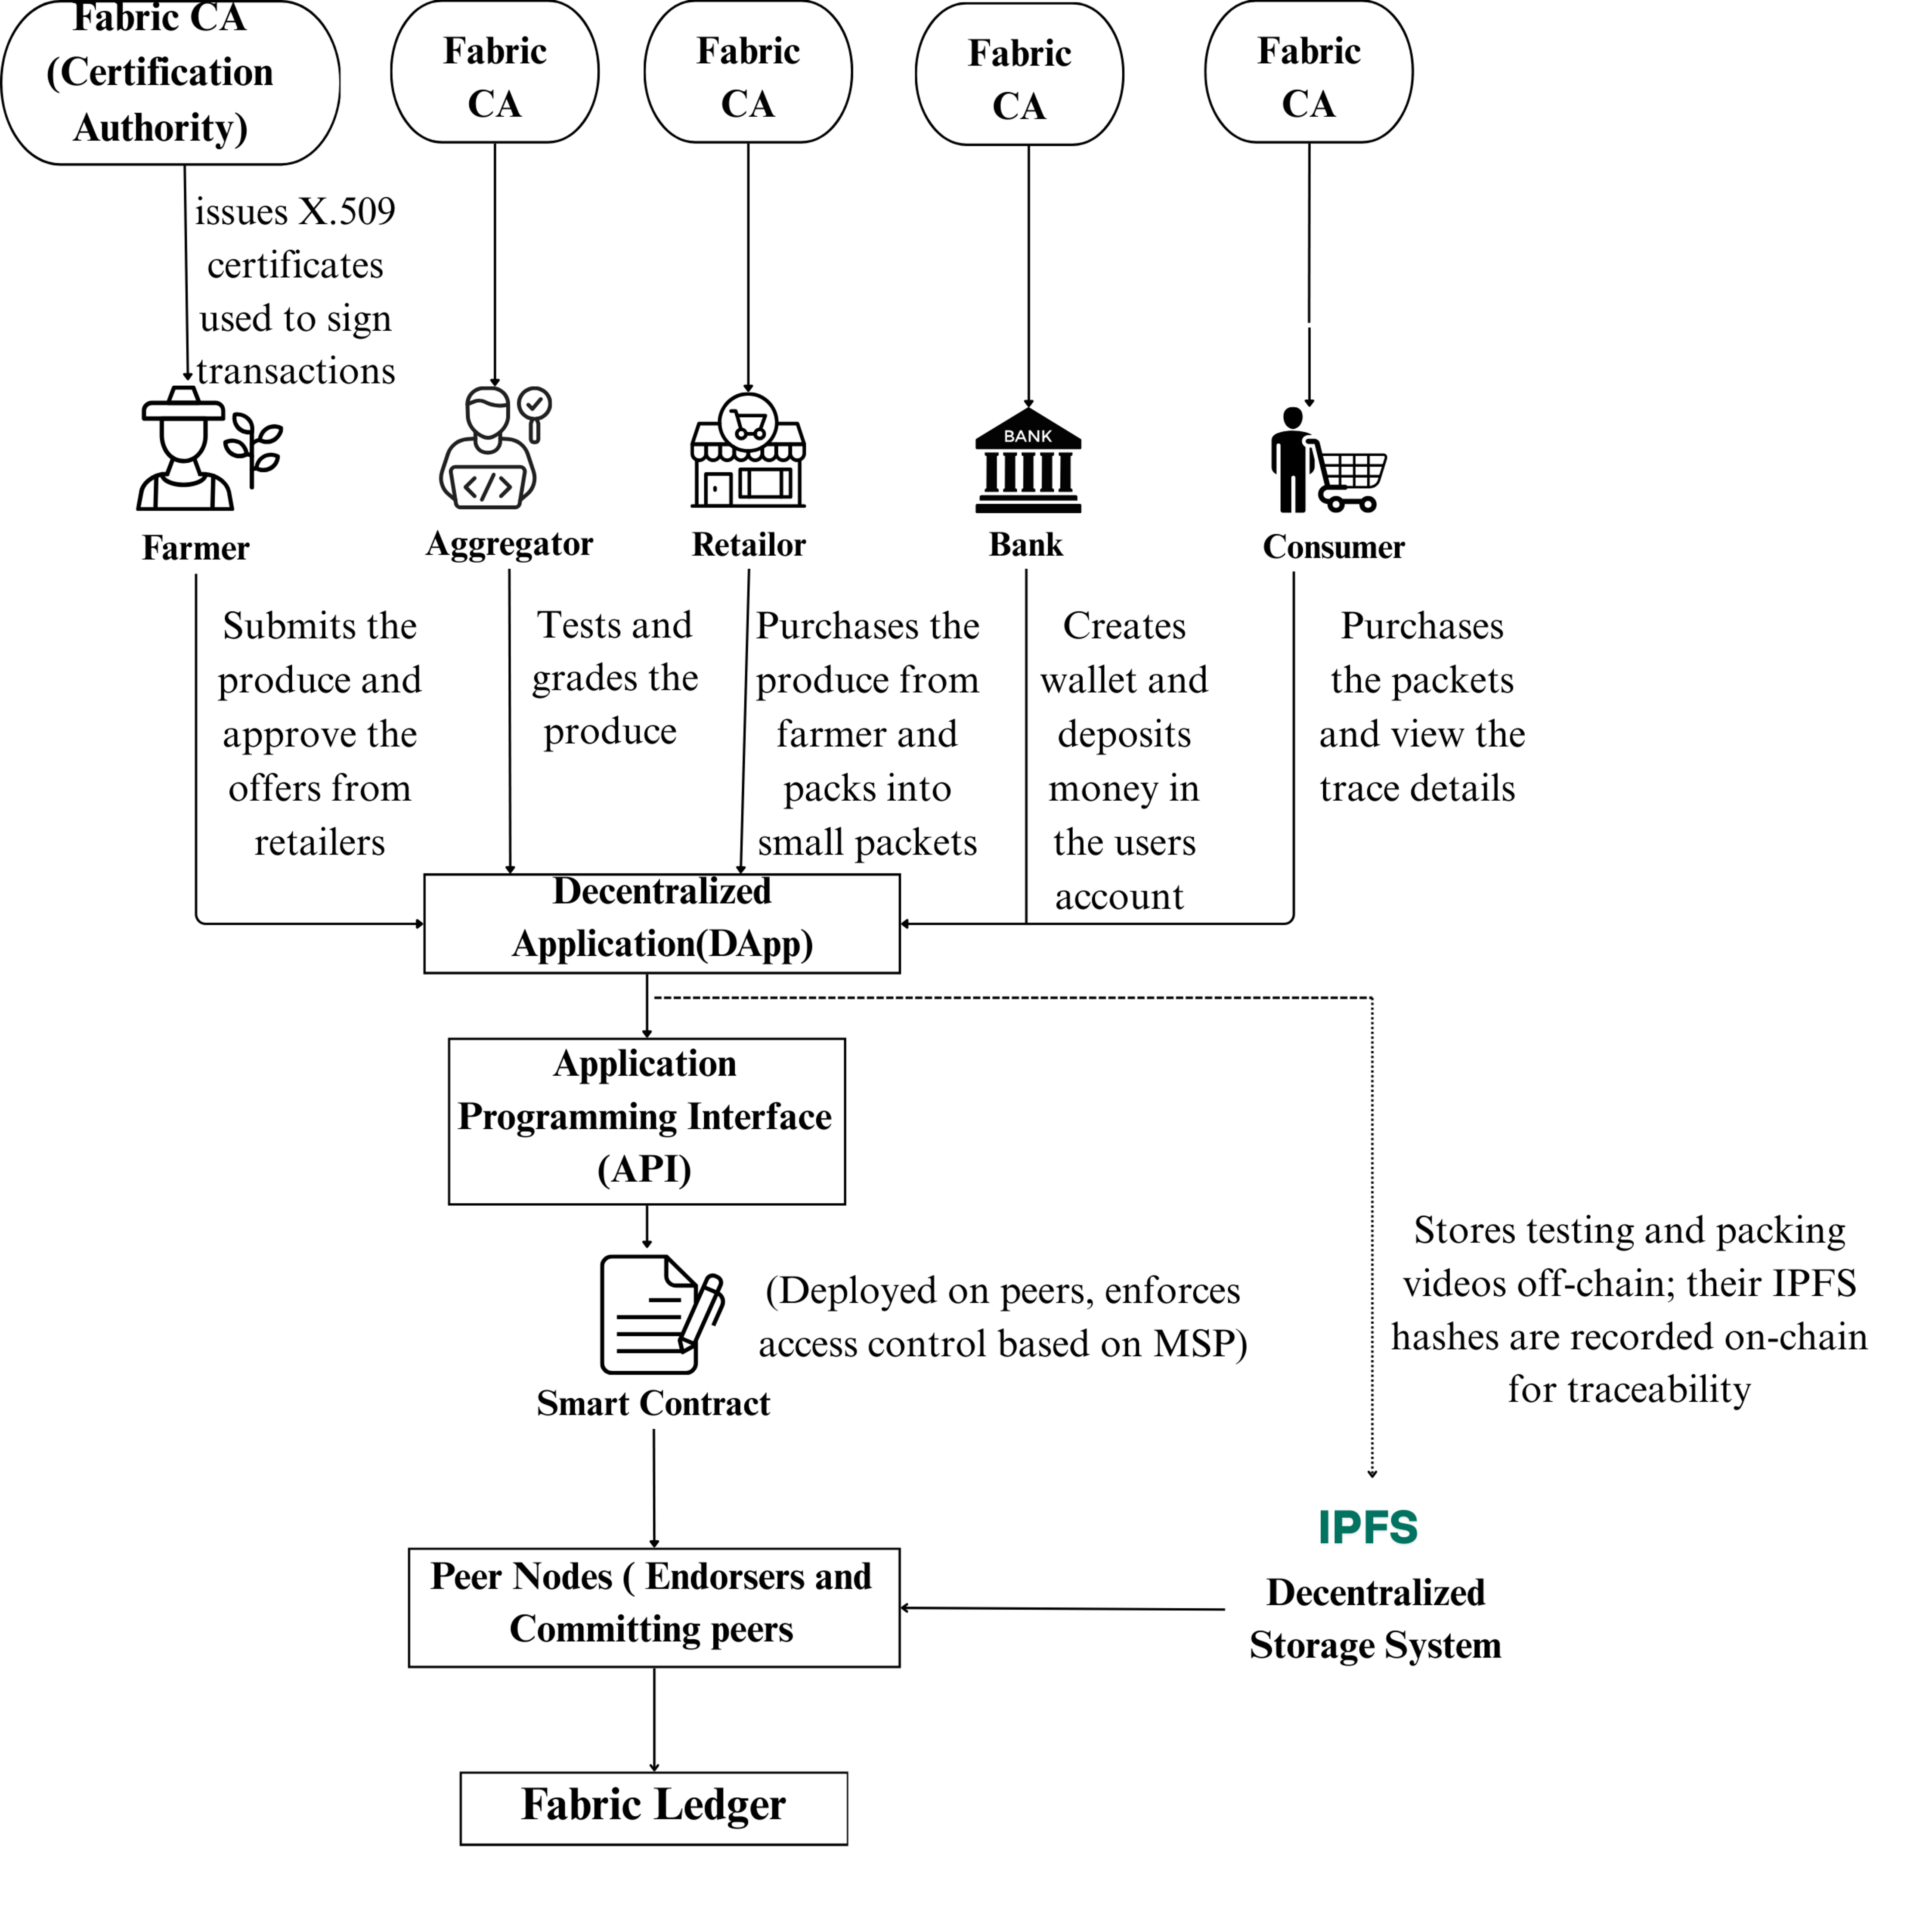
\includegraphics[width=0.9\textwidth]{Figure_1.png}
	\caption{System overview of the proposed agricultural supply chain platform}
	\label{fig:system_overview}
\end{figure}
	
	\subsection{Blockchain Network Architecture}
	
	The blockchain network was implemented using Hyperledger Fabric with five organizations: FarmersMSP, AggregatorsMSP, RetailersMSP, ConsumersMSP, and BankMSP. Each organization was configured with its own peer, MSP, and certificate authority. The organizations interact through a common channel, while CouchDB stores the world state. The network was created by extending the Fabric test network using customized Docker Compose, crypto-configuration, and channel configuration files. Raft was used as the ordering mechanism.
	
	
	\begin{figure}[htbp]
		
		\centering
		
		
\includegraphics[width=\textwidth]{Figure_2.png}
		
		\caption{Network Architecture}
		
		\label{fig:network_peer}
		
	\end{figure}
	
\subsection{Smart Contract Workflow}

The business logic was implemented as JavaScript chaincode. The bank creates and funds wallets using \texttt{createAccount}. Farmers submit lots via \texttt{createLot}, and aggregators update quality status using \texttt{testQuality}. Retailers bid via \texttt{makeOffer}, and the highest bidder executes \texttt{purchaseLot}, transferring funds automatically from their wallet to the farmer's wallet. Retailers repackage purchased lots using \texttt{createPacket}. Key features include: \texttt{createWallet()} and \texttt{depositMoney()}. Farmers submit agricultural lots using \texttt{submitProduce()}, and the testing fee is transferred to the selected aggregator. Aggregators record quality test results and grading details using \texttt{testQuality()}. Approved lots are made available for retailer offers through \texttt{makeOffer()}, and farmers accept the highest valid offer using \texttt{acceptOffer()}. Retailers then pack accepted lots into packets using \texttt{packLotIntoPackets()}, while consumers purchase packets using \texttt{purchasePacket()} and verify provenance through lifecycle query functions. The overall sequence of stakeholder actions and smart contract functions is shown in Figure~\ref{fig:chaincode_flow}.

\begin{figure}[htbp]
	\centering
	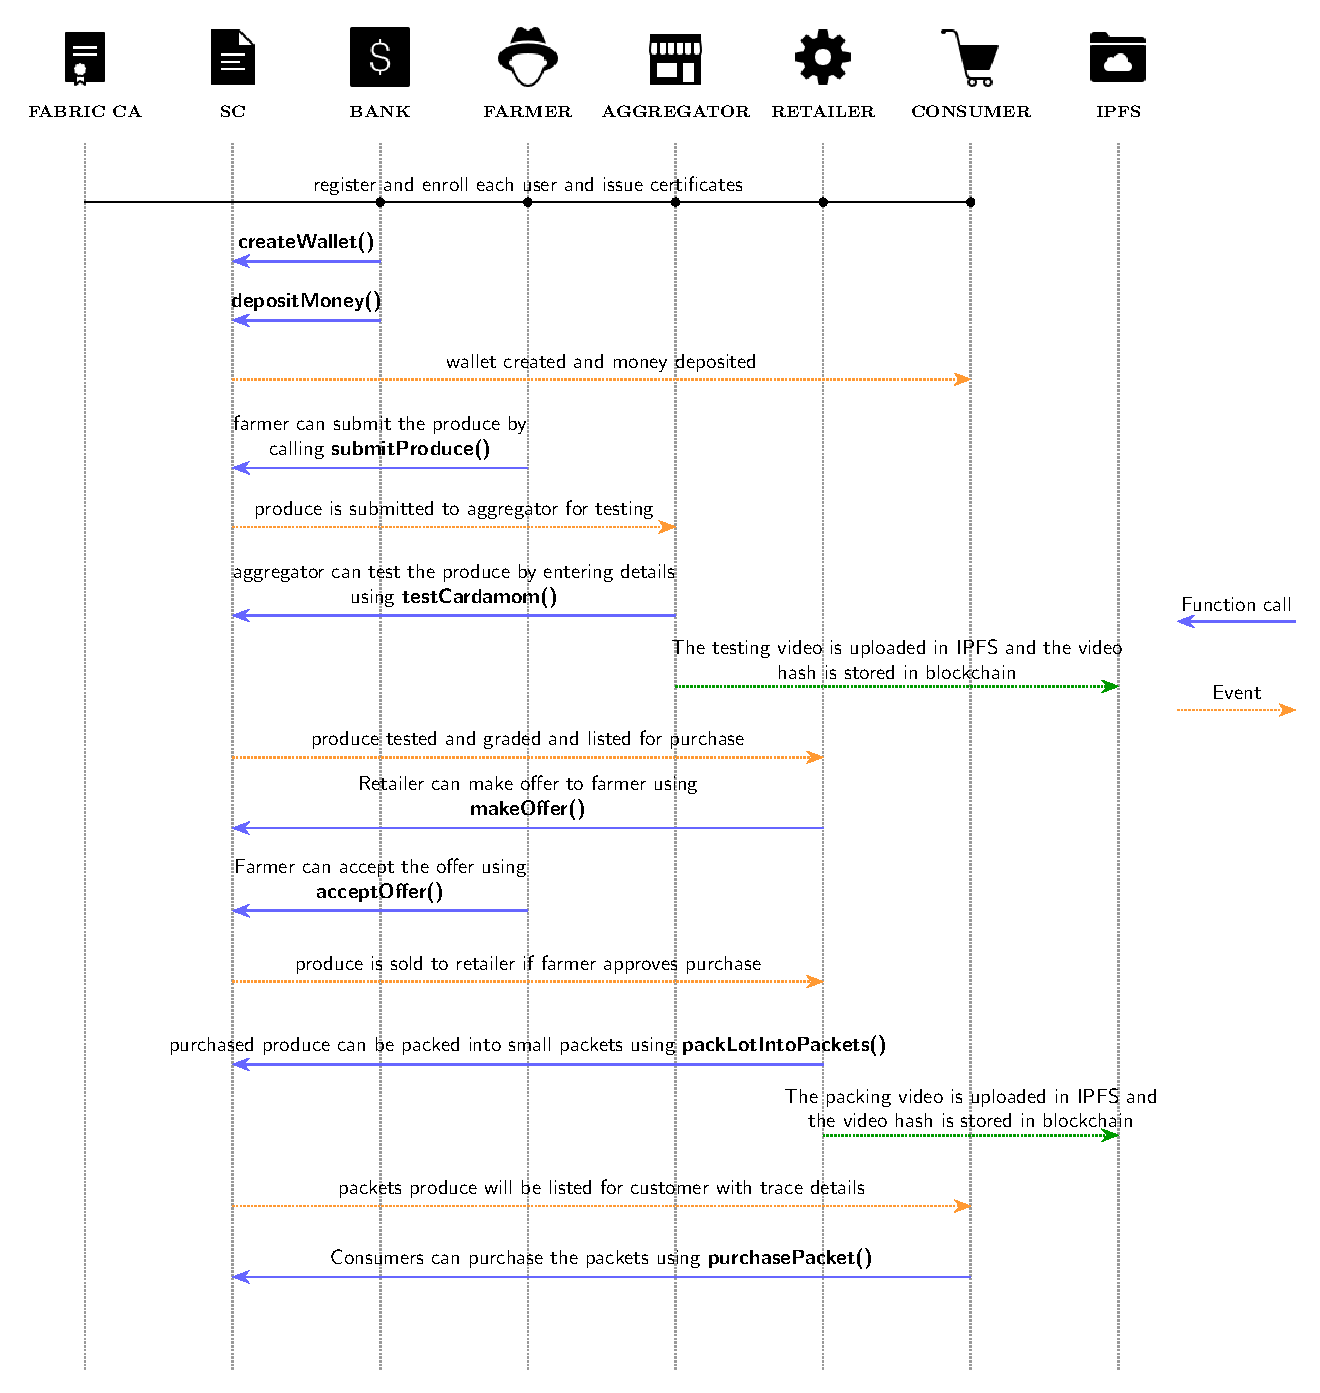
\includegraphics[width=\textwidth]{Figure_3.pdf}
	\caption{Sequence of stakeholder actions and smart contract functions in the agricultural supply chain}
	\label{fig:chaincode_flow}
\end{figure}

\subsubsection{Traceability, Auction, and Incentive Mechanism}

The traceability mechanism links each crop packet to its original lot, test result, grading details, and packing record. Testing and packing videos are stored off-chain in IPFS, while their hashes are stored on-chain for tamper-proof verification. This allows consumers to verify the product history using the packet code.

The auction mechanism supports price discovery for approved lots. Retailer offers are stored as separate composite-key records instead of being written into the lot record. This design choice is critical from an MVCC perspective: by giving each offer its own unique composite key, concurrent retailer bids no longer update the same shared lot state, thereby reducing MVCC contention. After the farmer accepts the highest valid offer, the smart contract transfers payment from the retailer wallet to the farmer wallet and updates lot ownership.

The incentive mechanism links quality compliance with farmer reputation. Approved lots improve the farmer rating and increase visibility to retailers, while rejected lots reduce the rating. This encourages farmers to follow quality-compliant cultivation practices and improves the credibility of producers. The integration of traceability, auction-based price discovery, and quality-compliance-based incentives is illustrated in Figure~\ref{fig:rating-incentive}.

\begin{figure}[H]
	\centering
	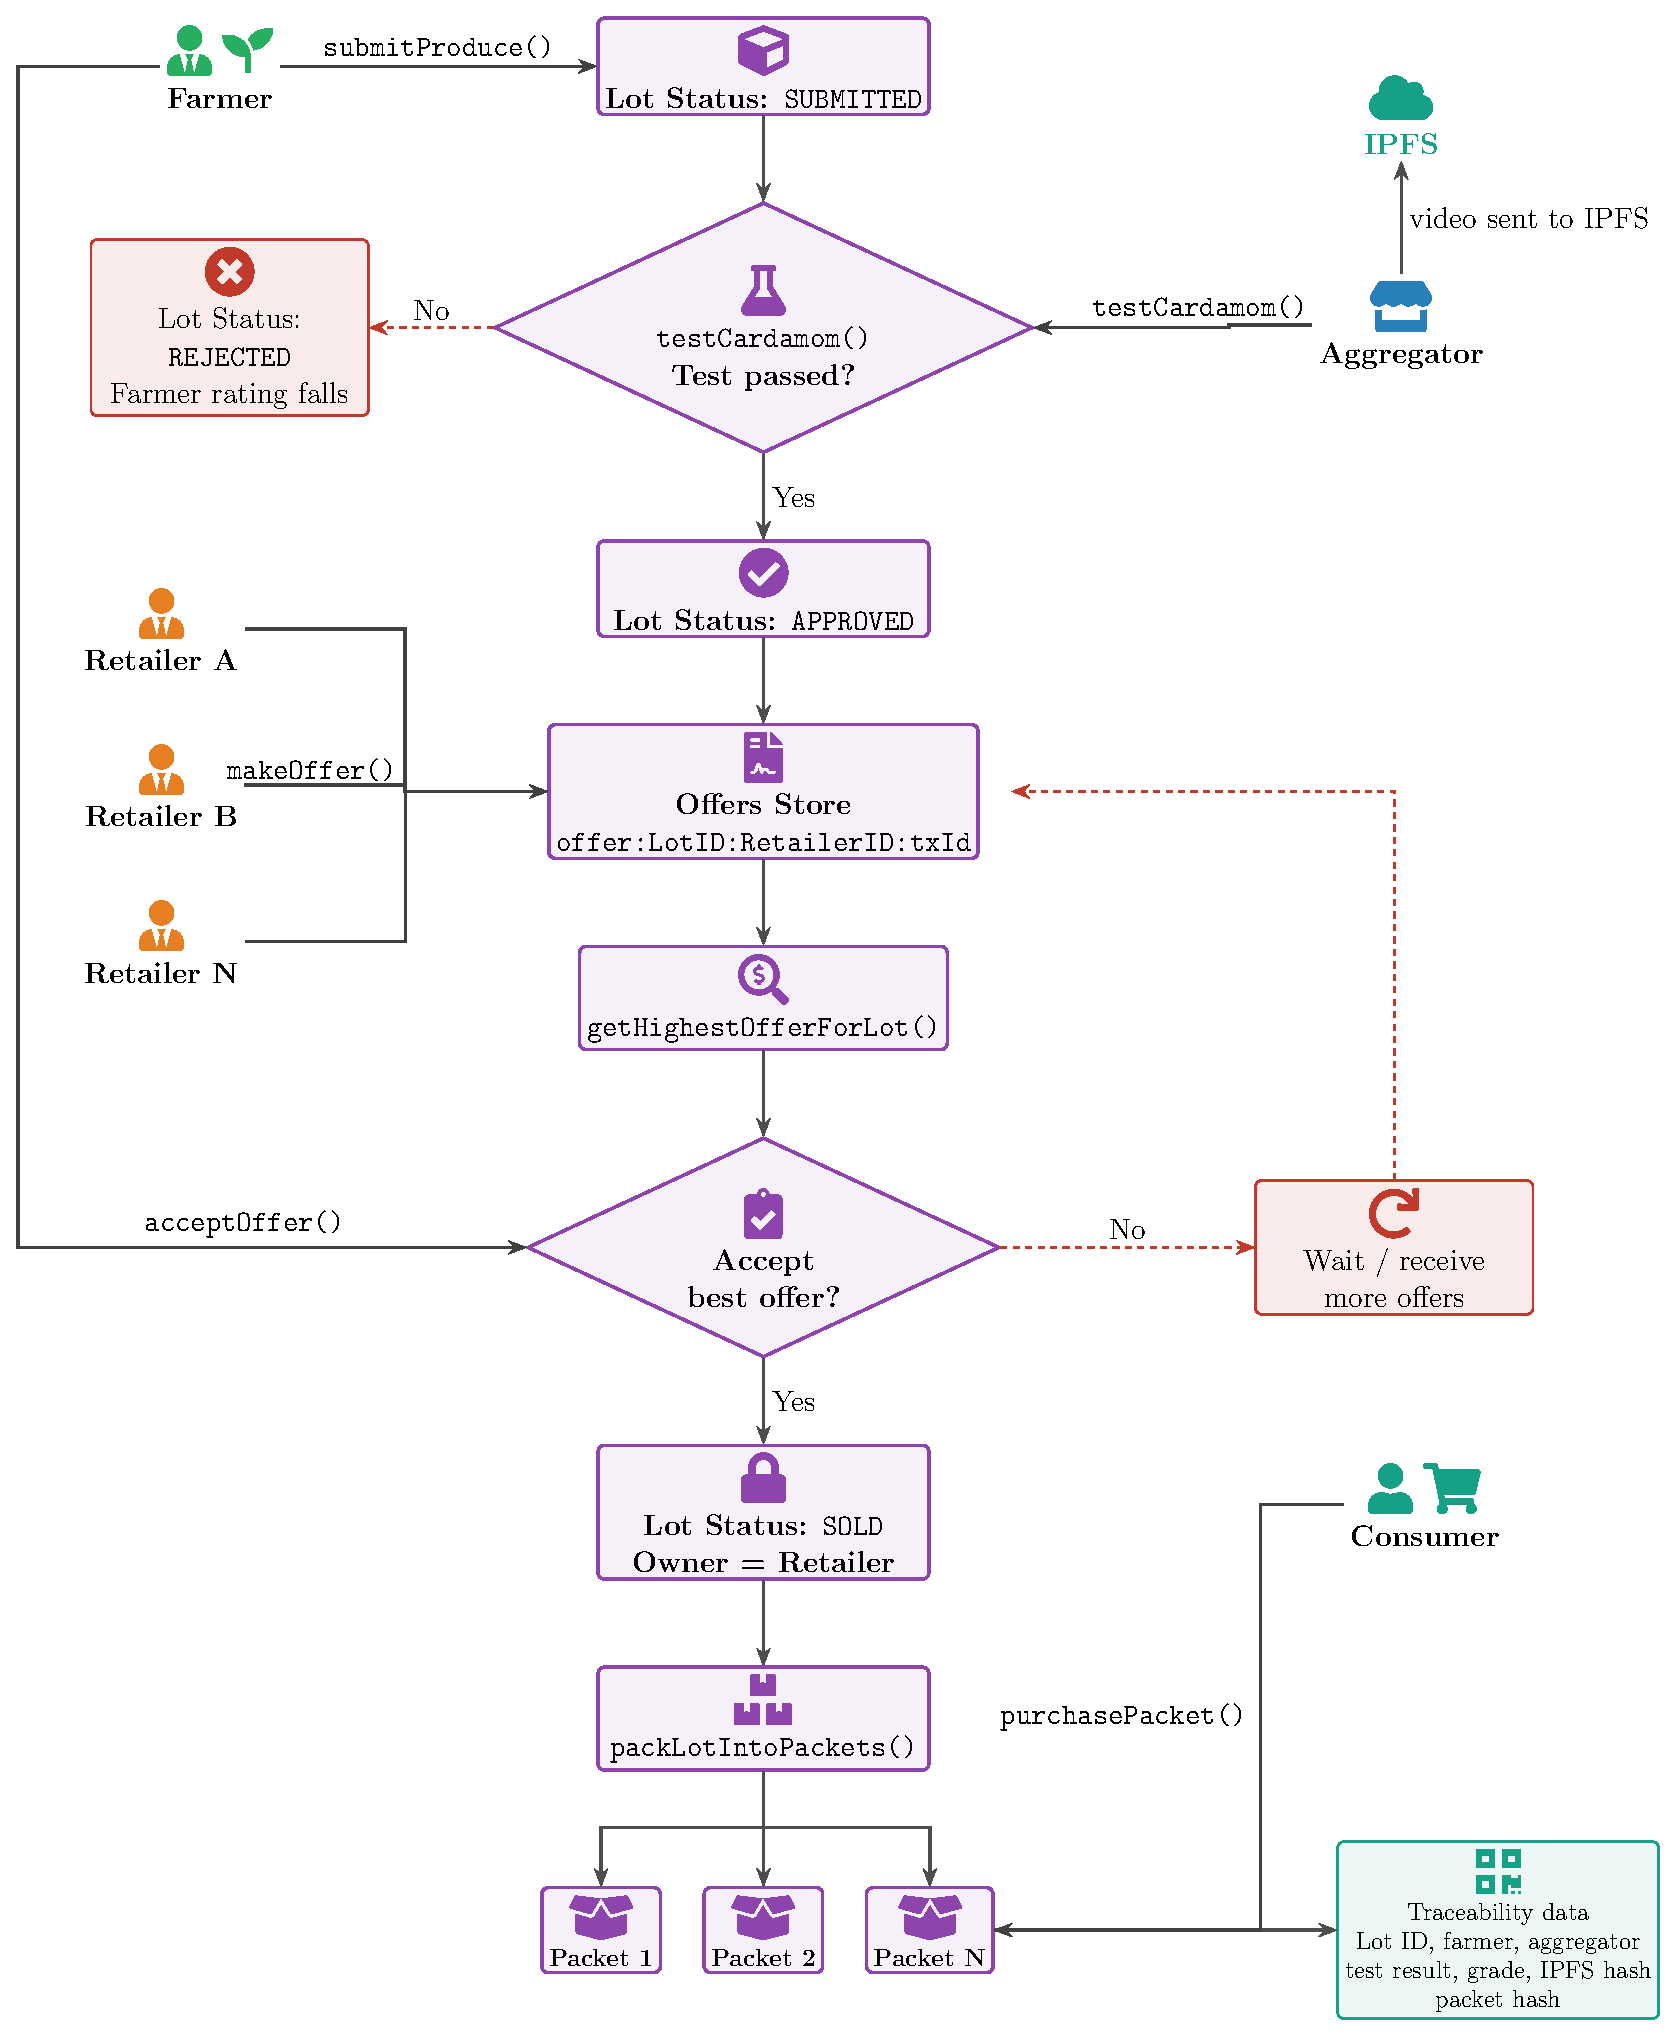
\includegraphics[width=0.95\textwidth]{Figure_4.pdf}
	\caption{Traceability, auction, and quality-compliance-based incentive mechanism}
	\label{fig:rating-incentive}
\end{figure}
	\subsection{Application Layer and IPFS Integration}
	
	A React.js web application was developed with separate dashboards for farmers, aggregators, retailers, consumers, and the bank. The frontend communicates with a Node.js backend through REST APIs. The backend invokes chaincode functions using the Fabric Gateway SDK and communicates with Fabric peers through gRPC. Large files, such as testing and packing videos, are stored off-chain in IPFS. The generated IPFS content identifier is stored on-chain with the corresponding lot or packet record, allowing users to verify external evidence without increasing blockchain storage overhead.
	
	
	\begin{figure}[!t]
		\centering
		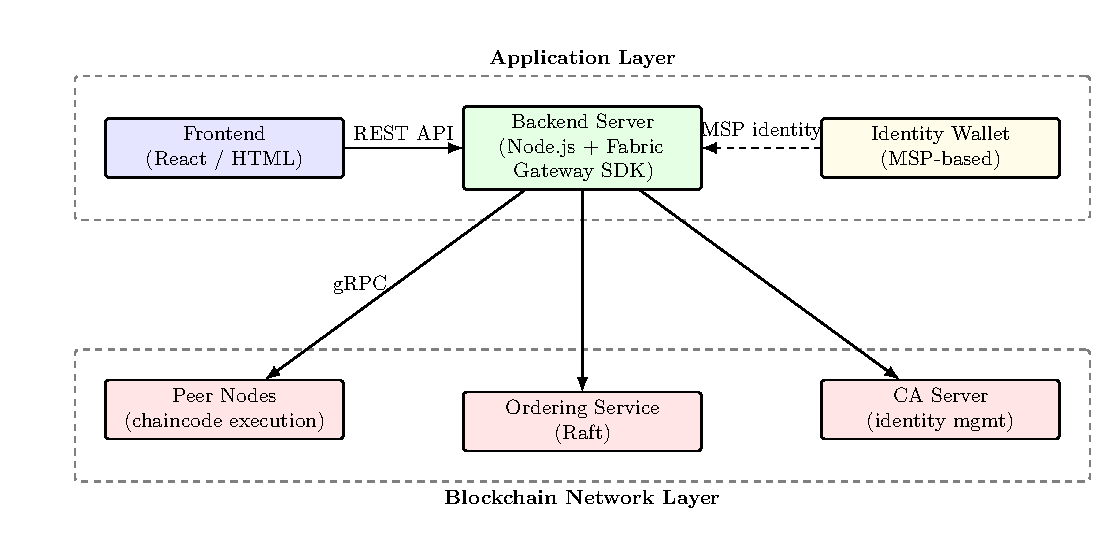
\includegraphics[width=190mm]{Figure_5.pdf}
		\caption{Interaction between Frontend, Fabric SDK, and the Hyperledger Fabric Network}
		\label{fig:fabric-interaction}
	\end{figure} 
	
	

\subsection{MVCC Conflict Vulnerabilities}

In high-throughput environments, the unoptimized chaincode is highly susceptible to Multi-Version Concurrency Control (MVCC) conflicts. Hyperledger Fabric employs an optimistic concurrency model: transactions are executed, endorsed, and ordered before validation against the ledger state. During the validation phase, if the version of a state key read during execution does not match the current committed version on the ledger, the transaction is marked invalid (MVCC \texttt{READ\_CONFLICT}) and abruptly dropped. In this supply chain design, there are two primary architectural bottlenecks where these conflicts predominantly occur:

\begin{enumerate}
    \item \textbf{Wallet Edits (\textit{submitProduce}, \textit{acceptOffer}, \textit{purchasePacket}):} Functions that facilitate financial transactions inherently invoke a shared internal \texttt{\_transfer} method. This method reads the current wallet balances of the sender and receiver, computes the new balances, and executes a \texttt{putState} operation to overwrite them. When multiple participants interact with a single entity concurrently (e.g., 50 farmers simultaneously submitting produce to a single aggregator), all 50 transactions read the exact same initial version of the aggregator's wallet key. The first transaction to successfully commit will increment the ledger version of that wallet. Consequently, the remaining 49 transactions will fail validation, severely throttling throughput.
    
    \item \textbf{Lot Highest Offer Edits (\textit{makeOffer}):} The auction mechanism allows multiple retailers to bid on an available agricultural lot concurrently. The \texttt{makeOffer} function reads the lot's current \texttt{highestOffer} parameter, validates if the new incoming bid is strictly greater, and overwrites the lot state. If multiple retailers bid on the exact same lot within the same block generation window, only the first endorsed transaction will successfully commit the updated lot state. The subsequent bids will encounter an MVCC conflict on the lot's shared composite key, causing those transactions to fail regardless of whether their bid values were objectively higher.
\end{enumerate}

These structural vulnerabilities form the foundational basis for the machine learning predictive models developed in this study, explicitly linking function complexity and hot-key density to deterministic transaction failure rates.


\section{System Testing and Benchmarking Methodology}
To comprehensively evaluate the agricultural supply-chain smart contract under varying levels of concurrent traffic and participant densities, performance benchmarking was conducted using Hyperledger Caliper (v0.5.0). Caliper allows the systematic generation of synthetic workloads against the deployed network to measure throughput, latency, and resource utilization. The extracted empirical performance metrics were subsequently utilized to train a Random Forest model to predict transaction failures and system throughput.

\subsection{Performance Benchmarking with Hyperledger Caliper}

The performance of the blockchain network was rigorously evaluated using Hyperledger Caliper, the industry-standard benchmarking tool for blockchain frameworks. The primary objective was to observe the dynamic shifts in transaction throughput and failure rates in response to increasing transaction send rates, fluctuating participant density, varying chaincode function complexity, and the resulting Multi-Version Concurrency Control (MVCC) hot-key contention.

\subsubsection{Transaction Loads and Workload Functions}

To capture the full spectrum of system performance—from an idle baseline to extreme network saturation—the experiments were conducted across a sequence of fixed-rate Transaction Per Second (TPS) loads: 1, 2, 4, 8, 10, 20, 50, 100, 200, 400, and 500 TPS. The default transaction duration for each load level was maintained at 5 seconds, with specific bulk operations extended to 100 seconds to ensure steady-state measurements. The benchmarking suite tested multiple distinct chaincode functions to represent real-world supply chain workflows, including \textit{testQuality}, \textit{makeoffer}, \textit{acceptoffer}, \textit{pack}, and \textit{submitproduce}. Each of these functions possesses a different structural complexity in terms of the number of state reads and writes required, as well as the number of participants contending for the same ledger key.

\subsubsection{Strategic Participant Matrix and Dynamic Caliper Network Generation}

To evaluate the impact of concurrent user scaling without exhaustively testing redundant participant combinations, a strategic participant matrix was designed. The number of participants for key roles (e.g., Farmers, Aggregators, Retailers) was scaled across predefined thresholds: 1, 2, 5, 10, 15, 20, and 24. 

For functions requiring interactive multi-party dependencies (such as Farmers submitting produce to Aggregators), a two-dimensional participant matrix was generated. This approach ensured comprehensive coverage of both balanced and imbalanced participant distributions while avoiding redundant reverse pairs.

Caliper workers were dynamically allocated based on the specific workload parameters. For example, in a \textit{submitproduce} workload configured with 5 farmers and 24 aggregators (\textit{submitproduce\_f5\_a24}), Caliper explicitly spawned 5 parallel worker processes acting as independent farmers. During execution, each farmer process probabilistically targeted one of the 24 available aggregators, actively stressing the shared ledger state and inducing measurable MVCC conflicts on the specific aggregator hot-keys.

To optimize the benchmarking infrastructure, 
un.js dynamically generated a workload-specific Caliper network configuration file for each experimental round. This dynamic provisioning ensured that only the required organizational identities (e.g., \textit{User1} to \textit{User24} for Farmers and Retailers) were actively instantiated and loaded into memory, thereby isolating chaincode performance metrics from artificial client-side resource starvation.

\begin{table}[ht]
\centering
\caption{Benchmark Workload Configurations and Participant Mapping}
\label{tab:workload_mapping}
\resizebox{\columnwidth}{!}{%
\begin{tabular}{|l|l|l|c|}
\hline
\textbf{Workload Function} & \textbf{Primary Role} & \textbf{Caliper Workers} & \textbf{Participant Target Range} \\
\hline
\textit{submitproduce} & Farmers & $X$ (number of farmers) & Aggregators (1 to $Y$) \\
\textit{testQuality} & Aggregators & $N$ (number of aggregators) & N/A \\
\textit{makeoffer} & Retailers & $N$ (number of retailers) & N/A \\
\textit{acceptoffer} & Farmers & $X$ (number of farmers) & Retailers (1 to $Y$) \\
\textit{pack} & Retailers & $N$ (number of retailers) & N/A \\
\hline
\end{tabular}%
}
\end{table}


\subsection{Machine Learning Method and Procedure}

The empirical output logs generated by Hyperledger Caliper across all benchmarking permutations were consolidated and extracted to formulate the primary dataset for the machine learning pipeline.

\subsubsection{Static Analysis of Smart Contract Function Complexity}

To precisely quantify the computational and state-interaction overhead of the chaincode, a custom static analysis pipeline (\textit{analyzeComplexity}) was developed. This tool systematically parses the smart contract source code to extract deterministic operational metrics per function, including the total number of ledger reads (\textit{getState}), ledger writes (\textit{putState}), conditional branches, and iteration loops. Most importantly, the tool explicitly identifies the exact composite keys targeted during write operations (MVCC Write Keys). By defining these structural metrics (detailed in Table \ref{tab:function_complexity}), the machine learning model can definitively correlate transaction performance with the exact number of highly contested hot-keys updated per invocation.

\begin{table}[ht]
\centering
\caption{Static Analysis of Smart Contract Function Complexity and MVCC Hot-Keys}
\label{tab:function_complexity}
\resizebox{\columnwidth}{!}{%
\begin{tabular}{|l|c|c|c|}
\hline
\textbf{Function} & \textbf{Total Reads} & \textbf{Total Writes} & \textbf{MVCC Write Keys (Hot-Keys)} \\
\hline
\textit{submitProduce} & 3 & 3 & Wallet Balance (fromKey, toKey) \\
\textit{testQuality} & 1 & 1 & None \\
\textit{makeOffer} & 2 & 1 & lot.highestOffer \\
\textit{acceptOffer} & 3 & 3 & Wallet Balance (fromKey, toKey) \\
\textit{packLotIntoPackets} & 1 & 2 & None \\
\textit{purchasePacket} & 3 & 3 & Wallet Balance (fromKey, toKey) \\
\hline
\end{tabular}%
}
\end{table}
 
  \subsubsection{Mechanics of MVCC Hot-Key Contention}
  In Hyperledger Fabric, Multi-Version Concurrency Control (MVCC) ensures data integrity by preventing concurrent transactions from modifying the exact same ledger state simultaneously. A ``hot-key'' bottleneck occurs when multiple active clients attempt to update the same state variable (key) at the exact same moment. If multiple transactions target the same state variable in the same block window, the first transaction successfully commits, while all subsequent concurrent transactions are instantly rejected by the validation peers with an MVCC read-write conflict, resulting in transaction failure.
  
  In the context of the proposed agri-food smart contracts, these hot-key collisions mathematically dictate the failure rate and manifest in specific algorithmic patterns:
  \begin{itemize}
      \item \textbf{Wallet Balance Edits (\textit{acceptOffer}, \textit{purchasePacket}):} Functions that facilitate financial settlements require updating the wallet keys (e.g., \texttt{token\_balance}) of both the buyer and the seller. For instance, when multiple consumers simultaneously purchase items from a highly active retailer, the retailer's single wallet key becomes a massive congestion point, triggering severe MVCC conflicts.
      \item \textbf{Bidding on Shared Assets (\textit{makeOffer}):} When multiple retailers concurrently submit competitive bids on a single, highly desirable produce lot, the smart contract continuously attempts to update the \texttt{lot.highestOffer} parameter within the exact same \texttt{lotKey} state object. Consequently, only one bid can successfully commit per state version, drastically increasing the likelihood of rejection for all other concurrently executing bids.
  \end{itemize}
   
  
  \subsubsection{Data Collection and Feature Selection}

The dataset's features were carefully selected to capture the nonlinear interactions inherent in blockchain architecture that directly trigger transaction failures. Because MVCC failures in Hyperledger Fabric are predominantly caused by concurrent read/write operations on identical state keys, the selected independent variables explicitly quantified both the computational load and the specific state-write dependencies. The primary features included:
\begin{itemize}
    \item \textbf{Transaction Send Rate (Load):} The targeted number of transactions submitted per second.
    \item \textbf{Number of Caliper Workers:} The number of parallel client workers actively submitting transactions to the network simultaneously, directly dictating concurrent thread pressure.
    \item \textbf{Participant Density:} The explicit count of active Farmers, Aggregators, Retailers, Consumers, and Bank Users interacting with the smart contract.
    \item \textbf{Number of Ledger Writes:} Extracted directly from the \textit{analyzeComplexity} static analysis tool, this integer represents the absolute baseline structural complexity of the transaction. Rather than passing categorical function names, feeding the model the exact ledger write count allows it to mathematically correlate the underlying algorithmic topology to failure vulnerabilities.
    \item \textbf{Hot-Key Participant Count:} A derived feature representing the severity of concurrent operations on shared state keys. As identified during the functional analysis, during the \textit{submitProduce} function, both the farmers' and aggregators' wallet accounts are overwritten continuously. During \textit{makeOffer}, a specific lot's highest offer parameter is updated by competing retailers. Most critically, during \textit{acceptOffer}, the wallet accounts of both the farmer and the retailer are rewritten, explicitly exposing the transaction to two distinct, highly contended hot keys. The total count of participants interacting with these precise hot-keys directly affects the probability of MVCC failure.
    \item \textbf{Network Metrics:} Additional network infrastructure variables, including artificially injected network latency (ms), were logged when applicable.
\end{itemize}

To provide a comprehensive dataset for the machine learning model, the benchmarking framework generated permutations across these features using the parameter ranges defined in Table \ref{tab:experimental_ranges}.

\begin{table}[ht]
\centering
\caption{Experimental Benchmarking Parameter Ranges}
\label{tab:experimental_ranges}
\resizebox{\columnwidth}{!}{%
\begin{tabular}{|l|l|}
\hline
\textbf{Experimental Parameter} & \textbf{Evaluated Range / Values} \\
\hline
Transaction Send Rate (TPS) & 1, 2, 4, 8, 10, 20, 50, 100, 200, 400, 500 \\
Number of Caliper Workers & 1, 2, 5, 10, 15, 20, 24 \\
Participant Density Matrix & (1,1), (1,2), (1,5), (2,2), (2,5), (5,5) ... up to (24,24) \\
Transactions per Round & 500 fixed transactions per permutation \\
Workload Duration & Dynamic based on TPS, with specific caps (e.g., 100s) \\
Network Impairments & Baseline (0ms latency) \\
\hline
\end{tabular}%
}
\end{table}

\subsubsection{Predictive Modeling and Baseline Comparison}

To map the relationship between these system variables and the observed chaincode behavior, five distinct machine learning regression architectures were evaluated:
\begin{itemize}
    \item \textbf{Linear Regression:} Baseline linear correlation model.
    \item \textbf{Support Vector Regressor (SVR):} Distance-based regression mapping.
    \item \textbf{Multi-Layer Perceptron (MLP):} A standard Neural Network architecture.
    \item \textbf{Random Forest Regressor:} A tree-based ensemble method.
    \item \textbf{eXtreme Gradient Boosting (XGBoost):} An advanced, highly optimized tree-based boosting framework.
\end{itemize}

The selection of Random Forest as the primary predictive architecture was driven by the unique failure mechanics of Hyperledger Fabric and by the empirical model comparison results. Blockchain performance degradation---specifically MVCC read-write conflicts and throughput saturation---does not scale linearly. A network remains stable until a specific structural limit is hit, such as a critical mass of concurrent hot-key collisions or resource exhaustion, at which point performance can drop abruptly. Linear mapping models like Linear Regression and Support Vector Regression (SVR) are fundamentally limited for such threshold behavior. Tree-based ensemble methods create distinct conditional splits that better match the conditional transaction-validation logic of blockchain state machines. Random Forest was selected because it achieved strong predictive accuracy while retaining interpretable feature-importance estimates across throughput and failure-rate targets.

Crucially, rather than predicting the absolute number of failed transactions (which is artificially biased by the total number of transactions sent), the models were trained to predict the precise \textit{Failure Rate} (the percentage of failed transactions over the total submitted), alongside the successfully achieved system \textit{Throughput}.

\section{Results and Discussion}
\subsection{Functional Validation}

Functional validation was performed using both manual and automated testing. Manual testing was conducted through the web interface, REST API calls, and CLI commands to verify realistic stakeholder interactions. Automated scripts were then used to execute repeated transaction flows and confirm stable ledger updates.

The validation covered wallet creation and funding, produce submission, quality testing and grading, offer creation and acceptance, packet generation, consumer purchase, and provenance queries. Each transaction was followed by query operations to confirm correct state transitions, ownership updates, wallet changes, lot and packet status updates, and metadata consistency. Role-based access was tested using MSP identifiers to ensure that restricted functions could be invoked only by authorized stakeholders.

IPFS integration was validated by checking whether testing and packing video hashes were correctly stored on-chain and matched the corresponding off-chain files. These tests confirmed that the system preserved traceability and data consistency across the complete coffee supply chain workflow.

\subsection{Smart Contract Execution Summary}

Table~\ref{tab:smartcontract-validation} summarizes the main smart contract functions and their validated outcomes. The validation confirms that the implemented chaincode correctly supports wallet operations, produce submission, quality testing, auction-based offer handling, packetization, consumer purchase, and traceability verification.
	
	\begin{table}[ht]
		\centering
		\caption{Smart Contract Execution Validation}
		\label{tab:smartcontract-validation}
		\renewcommand{\arraystretch}{1.3}
		\begin{tabular}{|p{4cm}|p{9cm}|}
			\hline
			\textbf{Function} & \textbf{Validated Outcome} \\
			\hline
			\texttt{createWallet()}, \texttt{depositMoney()}  & Wallets were successfully created and token balances initialized for all stakeholders. \\
			\hline
			\texttt{submitProduce()} & Farmers submitted produce lots; testing fees were correctly deducted and transferred to aggregators. \\
			\hline
			\texttt{testQuality()}  & Test results and grading data were recorded; lot status updated based on quality score evaluation. \\
			\hline
			\texttt{makeOffer()}, \texttt{acceptOffer()} & Retailers submitted offers; farmers accepted valid offers and payments were transferred accordingly. \\
			\hline
			\texttt{packLotIntoPackets()} & Retailers generated traceable packets (100g–1kg) with associated metadata stored on-chain. \\
			\hline
			\texttt{purchasePacket()} & Consumers purchased packets and corresponding financial transactions were successfully executed. \\
			\hline
		\end{tabular}
	\end{table}
	

	
Overall, the validation confirmed that the system executed the intended stakeholder workflows correctly and maintained consistent ledger, wallet, and traceability records.
	
	
	
	
	

\subsection{Function-wise Write Performance}

Each core write function was evaluated independently under varying send rates using Hyperledger Caliper. The tested functions included \textit{submitProduce()}, \textit{testQuality()}, \textit{makeOffer()}, \textit{acceptOffer()}, \textit{packLotIntoPackets()}, and \textit{purchasePacket()}. The objective was to contextualize the empirical throughput and failure rates prior to machine learning analysis.

Table \ref{tab:baseline_performance} isolates the baseline network environment (0ms induced latency) to demonstrate how increasing concurrent load and client scaling distinctly affects different smart contract topologies. 

\begin{table}[ht]
\centering
\caption{Comprehensive Baseline Network Performance Profiles (0ms Latency)}
\label{tab:baseline_performance}
\resizebox{\columnwidth}{!}{%
\begin{tabular}{|l|c|c|c|c|c|}
\hline
\textbf{Function} & \textbf{Caliper Workers} & \textbf{Hot-Keys} & \textbf{Target Load (TPS)} & \textbf{Throughput (TPS)} & \textbf{Failure Rate} \\
\hline
submitproduce & 1 & 2 & 500 & 161.2 & 91.6\% \\
submitproduce & 10 & 20 & 500 & 278.2 & 98.1\% \\
submitproduce & 24 & 48 & 500 & 241.8 & 97.0\% \\
\hline
testQuality & 1 & 0 & 500 & 132.2 & 0.2\% \\
testQuality & 10 & 0 & 500 & 281.6 & 0.0\% \\
testQuality & 24 & 0 & 500 & 199.0 & 0.0\% \\
\hline
makeoffer & 1 & 1 & 500 & 235.9 & 46.6\% \\
makeoffer & 10 & 10 & 500 & 357.1 & 48.0\% \\
makeoffer & 24 & 24 & 500 & 341.8 & 48.0\% \\
\hline
acceptoffer & 1 & 2 & 500 & 0.0 & 0.0\% \\
acceptoffer & 10 & 20 & 500 & 39.6 & 87.6\% \\
acceptoffer & 24 & 48 & 500 & 38.9 & 88.7\% \\
\hline
pack & 1 & 0 & 500 & 0.0 & 0.0\% \\
pack & 10 & 0 & 500 & 0.0 & 0.0\% \\
pack & 24 & 0 & 500 & 0.0 & 0.0\% \\
\hline
purchase & 1 & 2 & 500 & 25.7 & 0.2\% \\
purchase & 10 & 20 & 500 & 243.0 & 99.0\% \\
purchase & 24 & 48 & 500 & 208.5 & 96.8\% \\
\hline
\end{tabular}%
}
\end{table}

Conversely, Table \ref{tab:latency_performance} illustrates the severe performance degradation introduced by wide-area network latency (10ms and 20ms) on a single function (\textit{submitproduce}).

\begin{table}[ht]
\centering
\caption{Impact of Network Latency on Throughput and Reliability (\textit{submitproduce})}
\label{tab:latency_performance}
\resizebox{\columnwidth}{!}{%
\begin{tabular}{|c|c|c|c|c|}
\hline
\textbf{Latency} & \textbf{Caliper Workers} & \textbf{Target Load (TPS)} & \textbf{Throughput (TPS)} & \textbf{Failure Rate} \\
\hline
10ms & 10 & 1 & 1.9 & 30.0\% \\
10ms & 5 & 500 & 244.0 & 99.4\% \\
\hline
20ms & 10 & 1 & 1.9 & 35.0\% \\
20ms & 5 & 500 & 230.2 & 99.5\% \\
\hline
\end{tabular}%
}
\end{table}

At 500 TPS, \textit{makeOffer()} achieved the best scalability among the tested write functions, maintaining very low average latency and reaching a maximum throughput of 416.3 TPS. This result reflects its lightweight design and reduced shared-state updates.

In contrast, more contention-prone operations exhibited higher latency and failure rates. The \textit{packLotIntoPackets()} function reached a throughput ceiling of about 140 TPS because each transaction creates multiple packet records, increasing endorsement and commit overhead. The \textit{purchasePacket()} function achieved high throughput but produced higher failure counts because multiple clients attempted to purchase the same packet concurrently, causing MVCC conflicts on the shared packet asset.

\subsection{Phase 2: Retrieval Function Benchmarking}

The second phase evaluated read-only functions, including \textit{getAllProduce()}, \textit{getAllPackets()}, and \textit{getPacketLifecycle()}. These functions do not modify ledger state but retrieve data using different access patterns. The \textit{getAllProduce()} and \textit{getAllPackets()} functions access the world state through composite-key scans and filtering, while \textit{getPacketLifecycle()} reconstructs provenance using transaction-history traversal.

Table~\ref{tab:getpacketlifecycle-loadtest} shows that \textit{getPacketLifecycle()} remained stable from 50 to 500 TPS, with no failures and very low average latency. Throughput closely followed the configured send rate, reaching 495.8 TPS at 500 TPS. This indicates that provenance queries can scale efficiently when history traversal is limited and no world-state updates are involved.

\begin{table}[h]
	\centering
	\caption{Performance Results for \texttt{getPacketLifecycle} (Payload: 2908 bytes) under Varying Load}
	\resizebox{\textwidth}{!}{
		\begin{tabular}{|l|c|c|c|c|c|c|c|c|}
			\hline
			Function & TPS & Total Tx & Failed & Send Rate & Max Lat (s) & Min Lat (s) & Avg Lat (s) & Throughput \\
			\hline
			getPacketLifecycle & 50  & 5000 & 0 & 50.0  & 0.06 & 0.00 & 0.01 & 50.0  \\
			getPacketLifecycle & 100 & 4995 & 0 & 99.9  & 0.02 & 0.00 & 0.01 & 99.9  \\
			getPacketLifecycle & 200 & 5000 & 0 & 199.8 & 0.50 & 0.01 & 0.01 & 199.8 \\
			getPacketLifecycle & 300 & 5000 & 0 & 299.4 & 0.03 & 0.01 & 0.01 & 299.3 \\
			getPacketLifecycle & 400 & 5000 & 0 & 377.8 & 1.19 & 0.00 & 0.01 & 373.6 \\
			getPacketLifecycle & 500 & 5000 & 0 & 496.2 & 0.10 & 0.00 & 0.02 & 495.8 \\
			\hline
		\end{tabular}
	}
	\label{tab:getpacketlifecycle-loadtest}
\end{table}

Table~\ref{tab:retrieval-combined} shows that world-state retrieval performance is strongly affected by payload size. Smaller payloads remained stable at lower and moderate loads, while larger payloads caused sharp latency growth, reduced throughput efficiency, and higher failure rates. This behaviour is mainly due to composite-key scanning, filtering, data serialization, and network transfer overhead. The results show that payload size is a major bottleneck for large read queries in Fabric-based supply chain applications.

The table presents the performance of both the \textit{getAllPackets()} and \textit{getProduce()} functions under varying payload sizes at a representative 100 TPS load. The results demonstrate a strong dependency of query performance on the volume of data retrieved.

For smaller payload sizes, the functions maintain stable performance with low latency and no failures. However, as the payload size increases significantly, performance degrades even at this moderate load level. Latency increases sharply and failure rates become substantial. Throughput drops considerably, reflecting the combined impact of expensive world-state traversal, large data serialization, and increased network transfer overhead. The larger response size prolongs request processing time, leading to accumulation of concurrent requests in the system.

This behaviour is primarily attributed to the increasing cost of world-state traversal, data aggregation, and response serialization as payload size grows. Since these functions rely on composite key scans and filtering operations over the world state, larger result sets significantly increase computational and I/O overhead. These results highlight that payload size is a dominant factor influencing read performance and that large-scale data retrieval can become a critical bottleneck in blockchain-based applications.

\begin{table}[h]
	\centering
	\caption{Performance Results for Retrieval Functions at 100 TPS under Varying Payload Sizes}
	\resizebox{\textwidth}{!}{
		\begin{tabular}{|l|c|c|c|c|c|c|c|}
			\hline
			\textbf{Function} & \textbf{Payload} & \textbf{TPS} & \textbf{Success} & \textbf{Failed} & \textbf{Send Rate} & \textbf{Avg Lat (s)} & \textbf{Throughput} \\
			\hline
			\texttt{getAllPackets} & 66 KB & 100 & 5000 & 0 & 100.0 & 0.01 & 99.9 \\
			\texttt{getAllPackets} & 330 KB & 100 & 5000 & 0 & 100.0 & 10.81 & 77.4 \\
			\texttt{getAllPackets} & 660 KB & 100 & 1049 & 3941 & 99.8 & 17.10 & 74.5 \\
			\hline
			\texttt{getProduce} & 94.3 KB & 100 & 4996 & 0 & 99.9 & 0.01 & 99.8 \\
			\texttt{getProduce} & 471.5 KB & 100 & 4215 & 785 & 100.1 & 32.32 & 55.2 \\
			\texttt{getProduce} & 943 KB & 100 & 427 & 4573 & 100.0 & 16.37 & 93.3 \\
			\hline
		\end{tabular}
	}
	\label{tab:retrieval-combined}
\end{table}
\subsection{Impact of Network Latency}

To examine the effect of network conditions, additional experiments were conducted by introducing controlled impairments between Docker containers: 50~ms fixed latency. Since the impact of network variability is more visible at higher loads, Table~\ref{tab:latency-500tps} reports the results at 500~TPS.

\begin{table}[h]
	\centering
	\caption{Performance Comparison of Smart Contract Functions at 500 TPS under Network Impairment}
	\resizebox{\textwidth}{!}{
		\begin{tabular}{|l|c|c|c|c|c|c|c|c|}
			\hline
			Function & TPS & Success & Failed & Send Rate & Max Lat (s) & Min Lat (s) & Avg Lat (s) & Throughput \\
			\hline
			submitProduce              & 500 & 4996 & 4    & 482.8 & 15.99 & 0.93 & 12.38 & 191.8 \\
			testQuality               & 500 & 4990 & 3    & 482.4 & 15.70 & 0.67 & 11.02 & 193.4 \\
			makeOffer                  & 500 & 5880 & 8    & 443.8 & 5.63  & 0.00 & 1.79  & 368.5 \\
			acceptOffer                & 500 & 4994 & 6    & 472.0 & 14.03 & 1.38 & 12.07 & 212.8 \\
			packLotIntoPackets         & 500 & 4993 & 7    & 590.0 & 70.15 & 19.83 & 62.74 & 70.51 \\
			purchasePacket             & 500 & 3346 & 1654 & 475.4 & 12.56 & 1.05 & 10.80 & 220.6 \\
			getProduce (13.2 KB)       & 500 & 804  & 4196 & 476.0 & 294.15 & 2.12 & 186.46 & 16.6 \\
			getAllPackets (66 KB)      & 500 & 1385 & 3613 & 483.5 & 293.78 & 1.05 & 223.76 & 16.5 \\
			\hline
		\end{tabular}
	}
	\label{tab:latency-500tps}
\end{table}

Table~\ref{tab:latency-500tps} shows that network impairment substantially increases latency and reduces throughput, especially for complex write operations and large retrieval queries. Functions such as \textit{submitProduce()}, \textit{testQuality()}, and \textit{acceptOffer()} show higher average latency because endorsement, ordering, and commit phases are all affected by communication delay. The \textit{packLotIntoPackets()} function is affected most among write operations due to write amplification from multiple packet records.

The \textit{makeOffer()} function remains comparatively stable, with lower latency and higher throughput, because it performs lightweight ledger updates. In contrast, \textit{purchasePacket()} shows higher failures because network delay increases the time window for concurrent access to the same packet asset, thereby increasing MVCC conflicts.

Retrieval functions show the strongest degradation under impaired network conditions. Both \textit{getProduce()} and \textit{getAllPackets()} involve larger response payloads, making them more sensitive to latency and peer-side request accumulation. The results indicate that read-path scalability is constrained by both payload size and request concurrency. Overall, the experiment confirms that network delay has a stronger impact on data-intensive and write-heavy functions than on lightweight transaction functions.
\subsection{Runtime Resource Utilization}

Table~\ref{tab:resource-combined} summarizes CPU, memory, and network I/O usage for representative write and retrieval functions. Write-intensive functions generally show increased CPU utilization at higher loads, especially \textit{packLotIntoPackets()} and \textit{acceptOffer()}, because they involve multiple state updates and ledger writes. In contrast, \textit{purchasePacket()} maintains relatively low CPU and memory usage, although its failures are mainly related to MVCC conflicts rather than resource exhaustion.

Retrieval functions show moderate CPU usage but higher network I/O, particularly for \textit{getAllPackets()} and \textit{getProduce()}, because they return larger payloads from the ledger. Memory usage remains stable across all functions, indicating that no abnormal memory growth or resource exhaustion occurred during benchmarking. Overall, the results suggest that the observed throughput and latency variations are mainly caused by transaction complexity, payload size, and concurrency effects rather than insufficient system resources.

\begin{table}[h]
	\centering
	\caption{Runtime Resource Utilization of Smart Contract and Retrieval Functions at 500 TPS Load}
	\resizebox{\textwidth}{!}{
		\begin{tabular}{|l|c|c|c|c|c|}
			\hline
			Function & TPS & CPU Avg (\%) & CPU Peak (\%) & Mem Avg (MB) & Net I/O (MB) \\
			\hline
			
			submitProduce & 500 & 26.58 & 82.8 & 369.37 & 7759.74 \\
			testQuality & 500 & 27.44 & 78.5 & 208.56 & 5865.42 \\
			acceptOffer & 500 & 28.86 & 81.7 & 371.74 & 8400.26 \\
			makeOffer & 500 & 25.54 & 86.0 & 297.45 & 2681.62 \\
			packLotIntoPackets & 500 & 38.19 & 85.0 & 379.52 & 7017.50 \\
			purchasePacket & 500 & 9.96 & 79.3 & 243.63 & 2577.23 \\
			getAllPackets & 500 & 21.58 & 69.2 & 340.15 & 6974.11 \\
			getProduce & 500 & 12.04 & 51.1 & 305.59 & 7657.60 \\
			getPacketDetails & 500 & 8.43 & 49.3 & 231.02 & 2586.68 \\
			\hline
			
		\end{tabular}
	}
	\label{tab:resource-combined}
\end{table}
	
\subsection{Optimization to Reduce MVCC Conflicts}

MVCC conflicts are a major source of transaction failure in Hyperledger Fabric when concurrent transactions update the same ledger key. In the unoptimized design, wallet transfers directly overwrote shared wallet-balance keys, while offer handling modified the same lot record during \textit{makeOffer()}. These read--modify--write patterns created shared-key contention under concurrent workloads.

To reduce these conflicts, the chaincode was redesigned using append-only records and composite keys. Wallet transfers were recorded as separate \texttt{walletTx} debit and credit entries instead of overwriting wallet balances. Retailer offers were also stored as independent \texttt{offer} assets using composite keys rather than being embedded in the lot record. This is achieved by moving the \texttt{getWalletBalance()} check outside the transfer function and the \texttt{getHighestOffer()} check outside \texttt{makeOffer()}. These validations need to be checked in the backend rather than in the chaincode. As a result, concurrent transactions generated unique ledger entries instead of repeatedly modifying shared state.

Table~\ref{tab:combined-performance} compares the unoptimized and optimized chaincode at 200~TPS. The optimized design substantially reduced transaction failures. For example, \textit{acceptOffer()} improved from 3963 failures to zero, while \textit{submitProduce()} improved from 3827 failures to zero. The \textit{makeOffer()} function also eliminated failures after separating offers from the lot record. Although \textit{purchasePacket()} still recorded 866 failures, this was mainly due to application-level contention where multiple clients attempted to purchase the same packet. Overall, the results confirm that append-only composite-key records significantly improve concurrency stability in the proposed Fabric system.


\begin{table}[h]
	\centering
	\caption{Performance Comparison of Unoptimized and Optimized Chaincode at 200 TPS}
	\resizebox{\textwidth}{!}{
		\begin{tabular}{|l|c|c|c|c|c|c|c|c|}
			\hline
			Function & TPS & Success & Fail & Send Rate & Max Lat (s) & Min Lat (s) & Avg Lat (s) & Throughput \\
			\hline
			
			\multicolumn{9}{|c|}{\textbf{Unoptimized Chaincode}} \\
			\hline
			
			acceptOffer & 200 & 1037 & 3963 & 200.1 & 2.20 & 0.08 & 0.99 & 199.8 \\
			makeOffer & 200 & 4630 & 380 & 200.4 & 2.05 & 0.00 & 0.05 & 185.5 \\
			packLotIntoPackets & 200 & 5000 & 0 & 200.0 & 13.91 & 0.25 & 12.79 & 109.1 \\
			purchasePacket & 200 & 1235 & 3765 & 199.4 & 2.84 & 0.05 & 0.10 & 179.4 \\
			submitProduce & 200 & 1173 & 3827 & 199.7 & 0.91 & 0 & 0.10 & 199.2 \\
			testQuality & 200 & 5000 & 0 & 199.9 & 0.73 & 0.04 & 0.10 & 199.5 \\
			
			\hline
			\multicolumn{9}{|c|}{\textbf{Optimized Chaincode}} \\
			\hline
			
			acceptOffer & 200 & 5000 & 0 & 199.2 & 1.49 & 0.00 & 0.12 & 198.7 \\
			makeOffer & 200 & 5010 & 0 & 199.6 & 2.04 & 0.00 & 0.05 & 185.0 \\
			packLotIntoPackets & 200 & 5000 & 0 & 199.5 & 17.17 & 0.19 & 10.73 & 118.9 \\
			purchasePacket & 200 & 4134 & 866 & 200.0 & 2.05 & 0.04 & 0.10 & 185.2 \\
			submitProduce & 200 & 5000 & 0 & 200.0 & 1.11 & 0.00 & 0.07 & 199.6 \\
			testQuality & 200 & 5000 & 0 & 199.8 & 0.15 & 0.00 & 0.08 & 199.4 \\
			
			\hline
		\end{tabular}
	}
	\label{tab:combined-performance}
\end{table}
	\subsection{Practical Implications and Limitations}
	
	The system is suitable for practical agricultural supply chain scenarios where transactions are usually asynchronous and occur at lower rates than the stress-test conditions. Under realistic operating loads, the system can support traceability, quality verification, auction-based price discovery, and smart contract-driven payments.
	
	However, the reported results should be interpreted as controlled laboratory measurements rather than production-scale throughput values. The experiments were conducted in a single-host Docker environment using WSL2, which does not fully capture wide-area network latency, geographically distributed endorsement, or multi-host ordering overhead. Future work should evaluate the system in a distributed deployment and optimize read-heavy functions through pagination, indexing, caching, and improved query design.
	
	\subsection{Machine Learning Predictive Insights}
	
	By training the machine learning pipeline on the empirical dataset, the models provided mathematical quantification of the underlying structural bottlenecks causing MVCC read-write conflicts. As detailed in the methodology, the models were blind to the categorical smart contract names and instead evaluated raw network load, client scaling, and the static \textit{Number of Ledger Writes} extracted via \textit{analyzeComplexity}.
	
	\subsubsection{Model Comparison and Feature Importance}
	To validate the hypothesis that MVCC conflicts scale non-linearly and exhibit threshold behavior based on structural topology, multiple regression architectures were evaluated and then checked against the latest Random Forest validation output. The Random Forest model achieved a testing $R^2$ of 0.9236 for throughput prediction and 0.9570 for failure-rate prediction, with corresponding MAE values of 11.933 and 0.0368. These values are consistent with the model-selection discussion in Section~\ref{tab:throughput_performance} and Section~\ref{tab:failure_performance}.
	
	The feature-importance results show two distinct bottleneck patterns. For throughput prediction, raw transaction load is the dominant variable, accounting for 81.1\% of predictive importance, followed by ledger writes (5.7\%), network latency (5.2\%), payload bytes (3.2\%), hot-key participants (2.5\%), and reads (2.4\%). For failure-rate prediction, hot-key participant density is dominant at 50.8\%, followed by payload bytes (20.5\%), transaction load (16.0\%), network latency (8.7\%), ledger writes (2.3\%), and reads (1.8\%). These results indicate that throughput is primarily governed by offered load, whereas MVCC failures are primarily governed by state-contention topology and are amplified by payload size, load, and latency.

	\subsubsection{Failure Analysis with Latency}

Network latency was found to exacerbate participant-level contention considerably. As latency increases, transactions require more time to complete their endorsement and commit cycles. During this extended processing window, the ledger keys involved in each transaction remain subject to potential conflict with other in-flight transactions. The longer this window, the greater the likelihood that subsequently submitted transactions will encounter stale state versions, resulting in MVCC read conflicts and rejection. At elevated latency levels, failure rates approached 100\% even at moderate transaction send rates.

\begin{figure}[H]
    \centering
    \begin{minipage}[b]{0.48\textwidth}
        \centering
        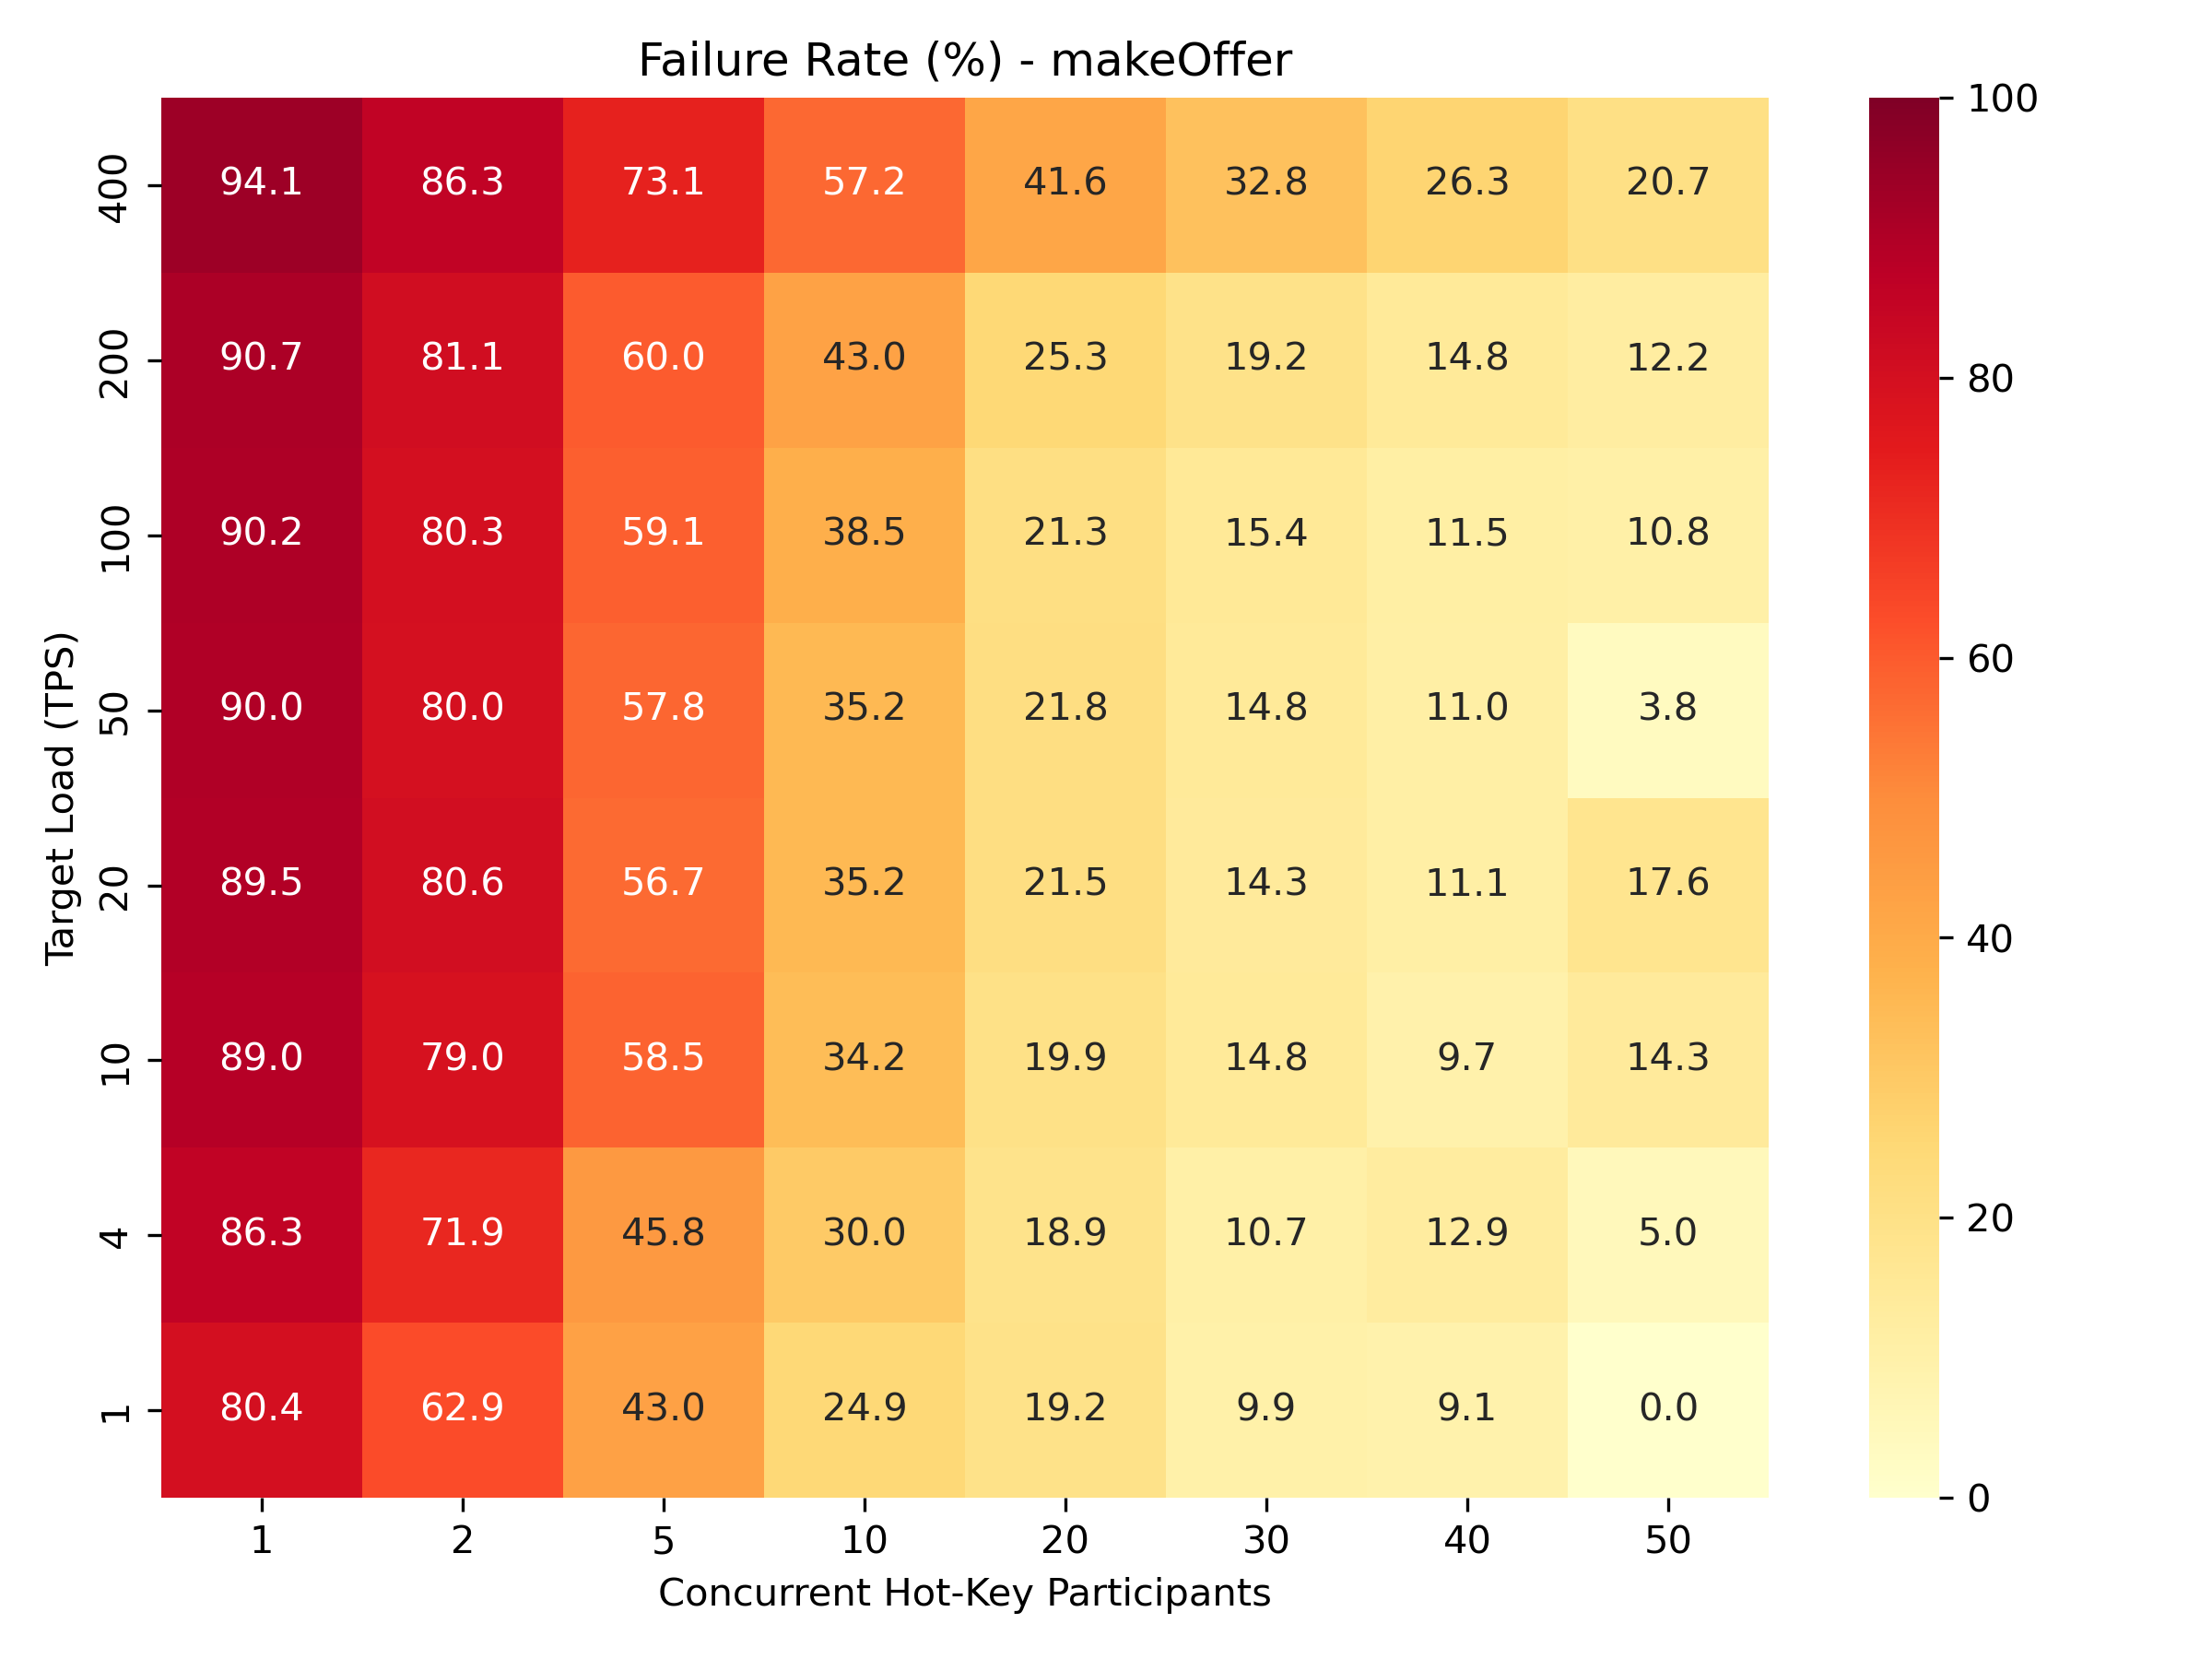
\includegraphics[width=\textwidth]{Figure_8a.png}
        \subcaption{makeOffer}
    \end{minipage}
    \hfill
    \begin{minipage}[b]{0.48\textwidth}
        \centering
        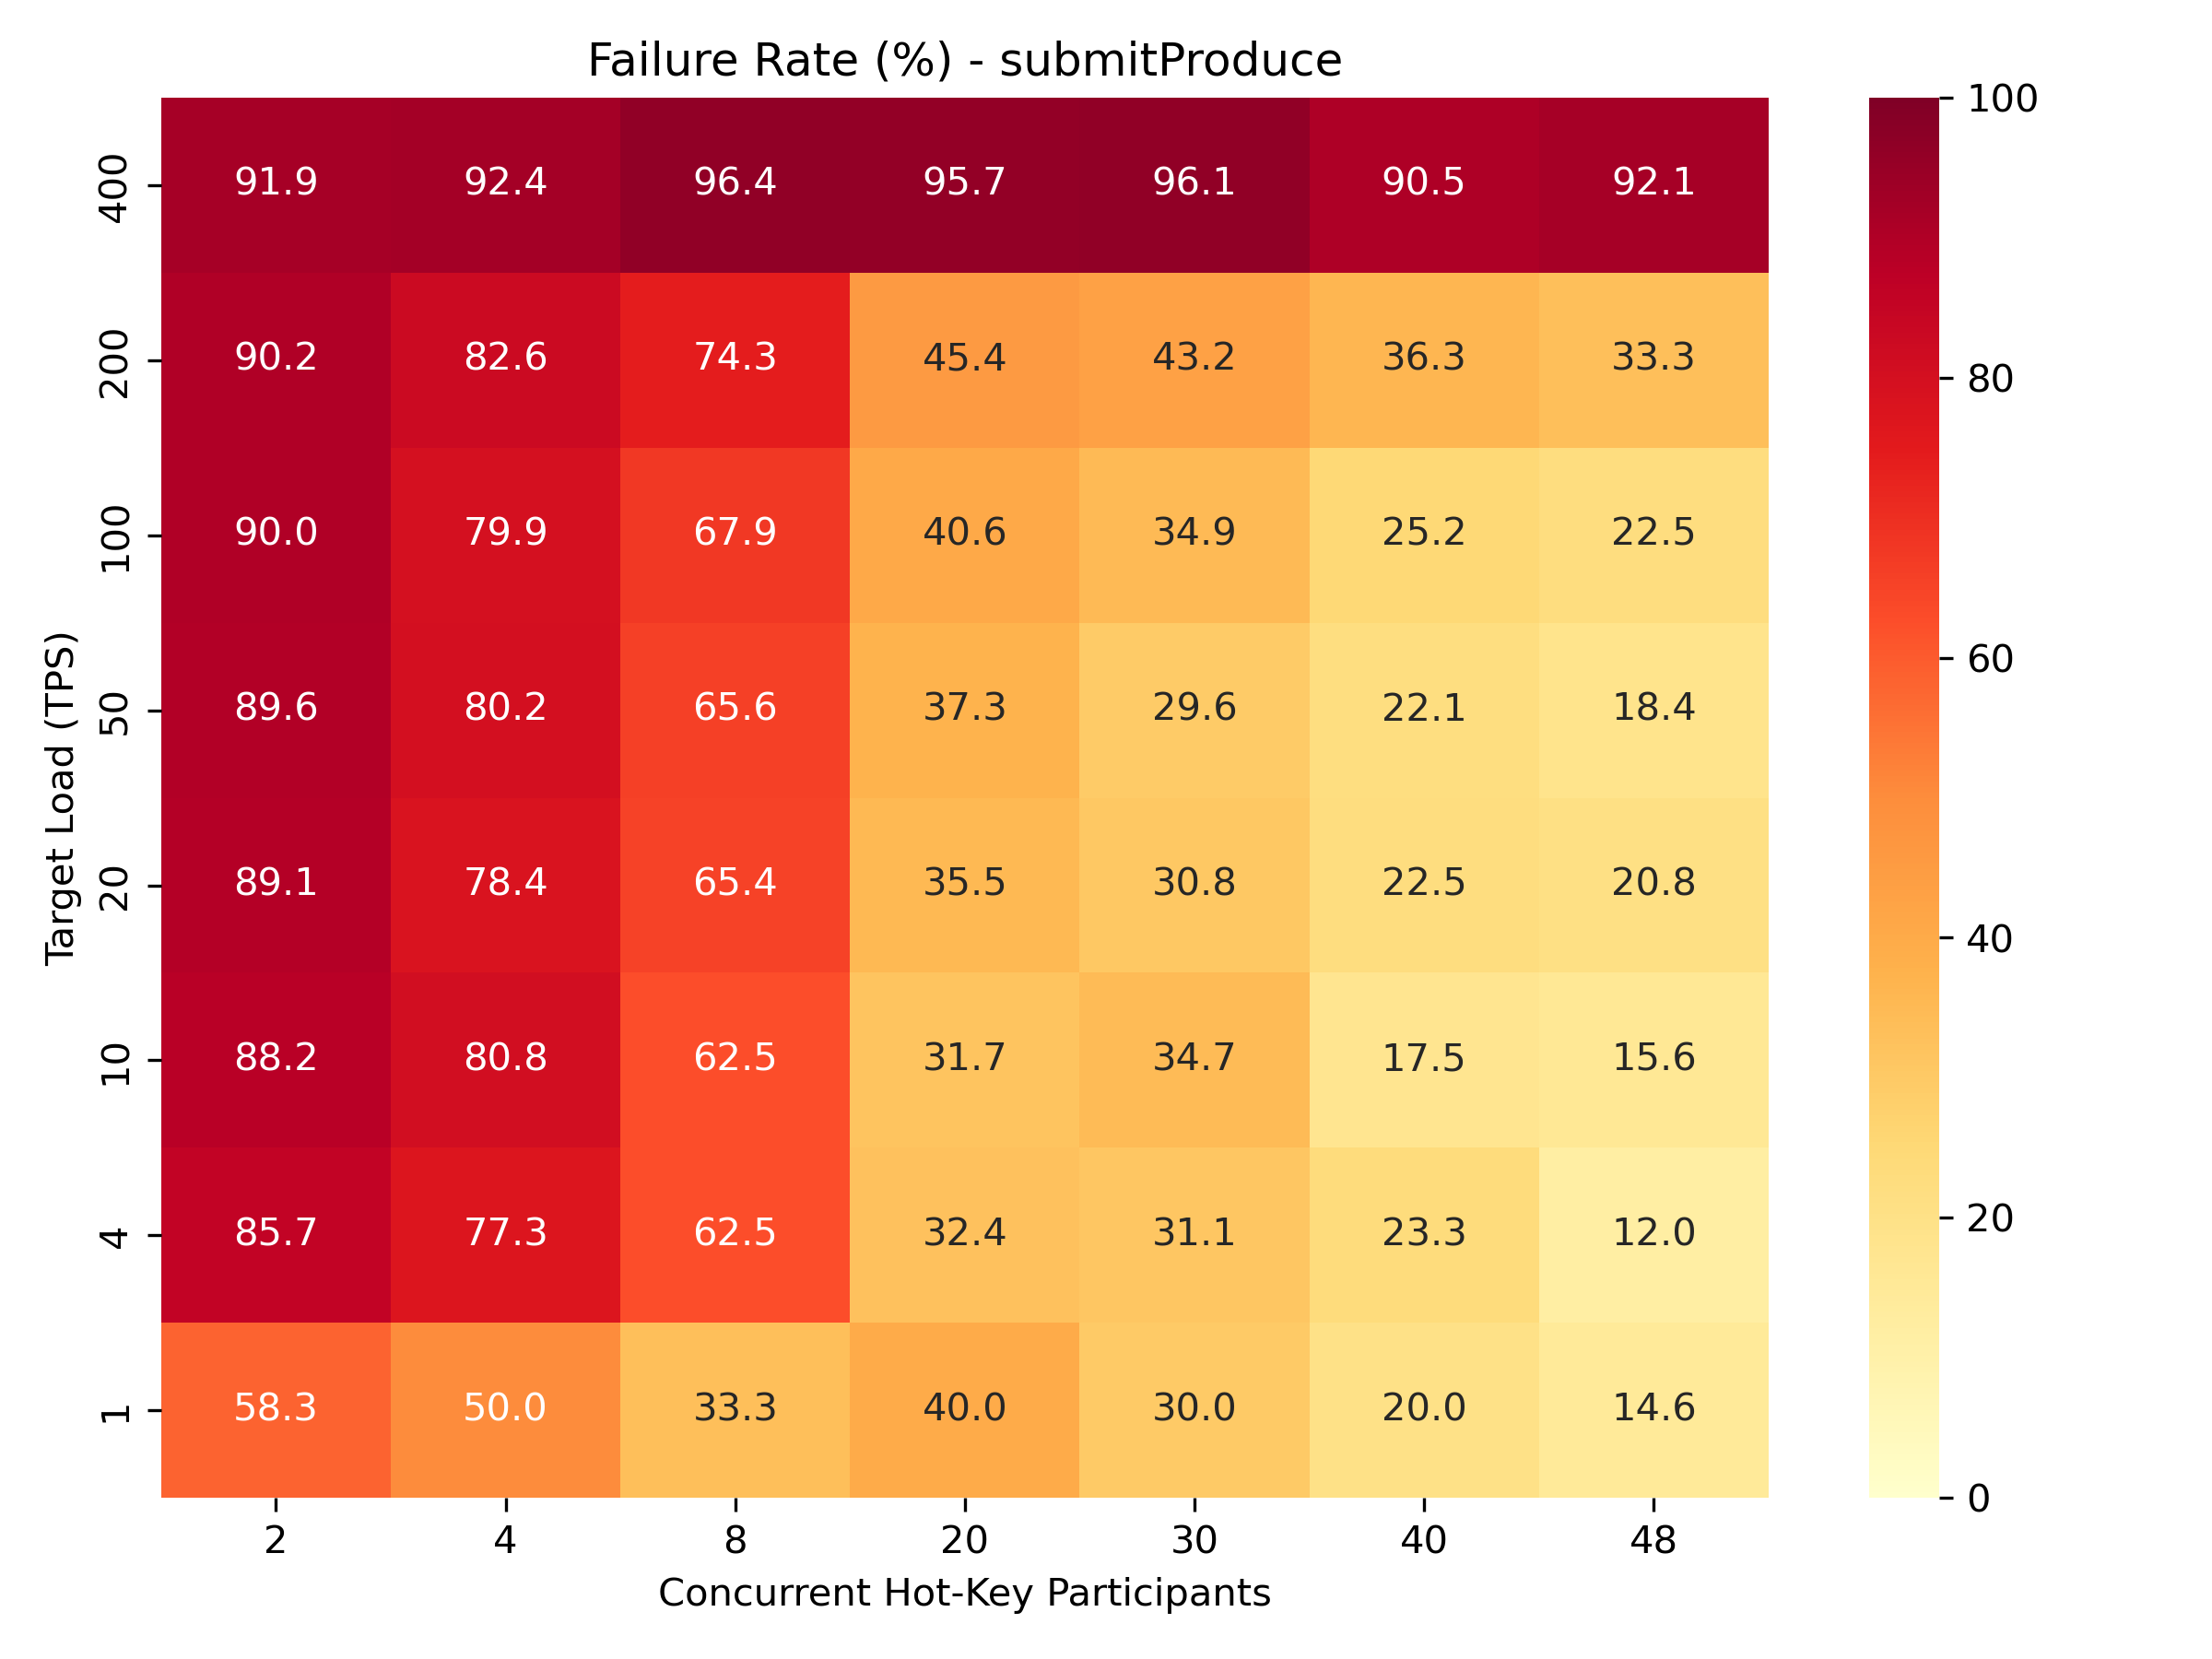
\includegraphics[width=\textwidth]{Figure_8b.png}
        \subcaption{submitProduce}
    \end{minipage}
    
    \vspace{0.3cm}
    
    \begin{minipage}[b]{0.48\textwidth}
        \centering
        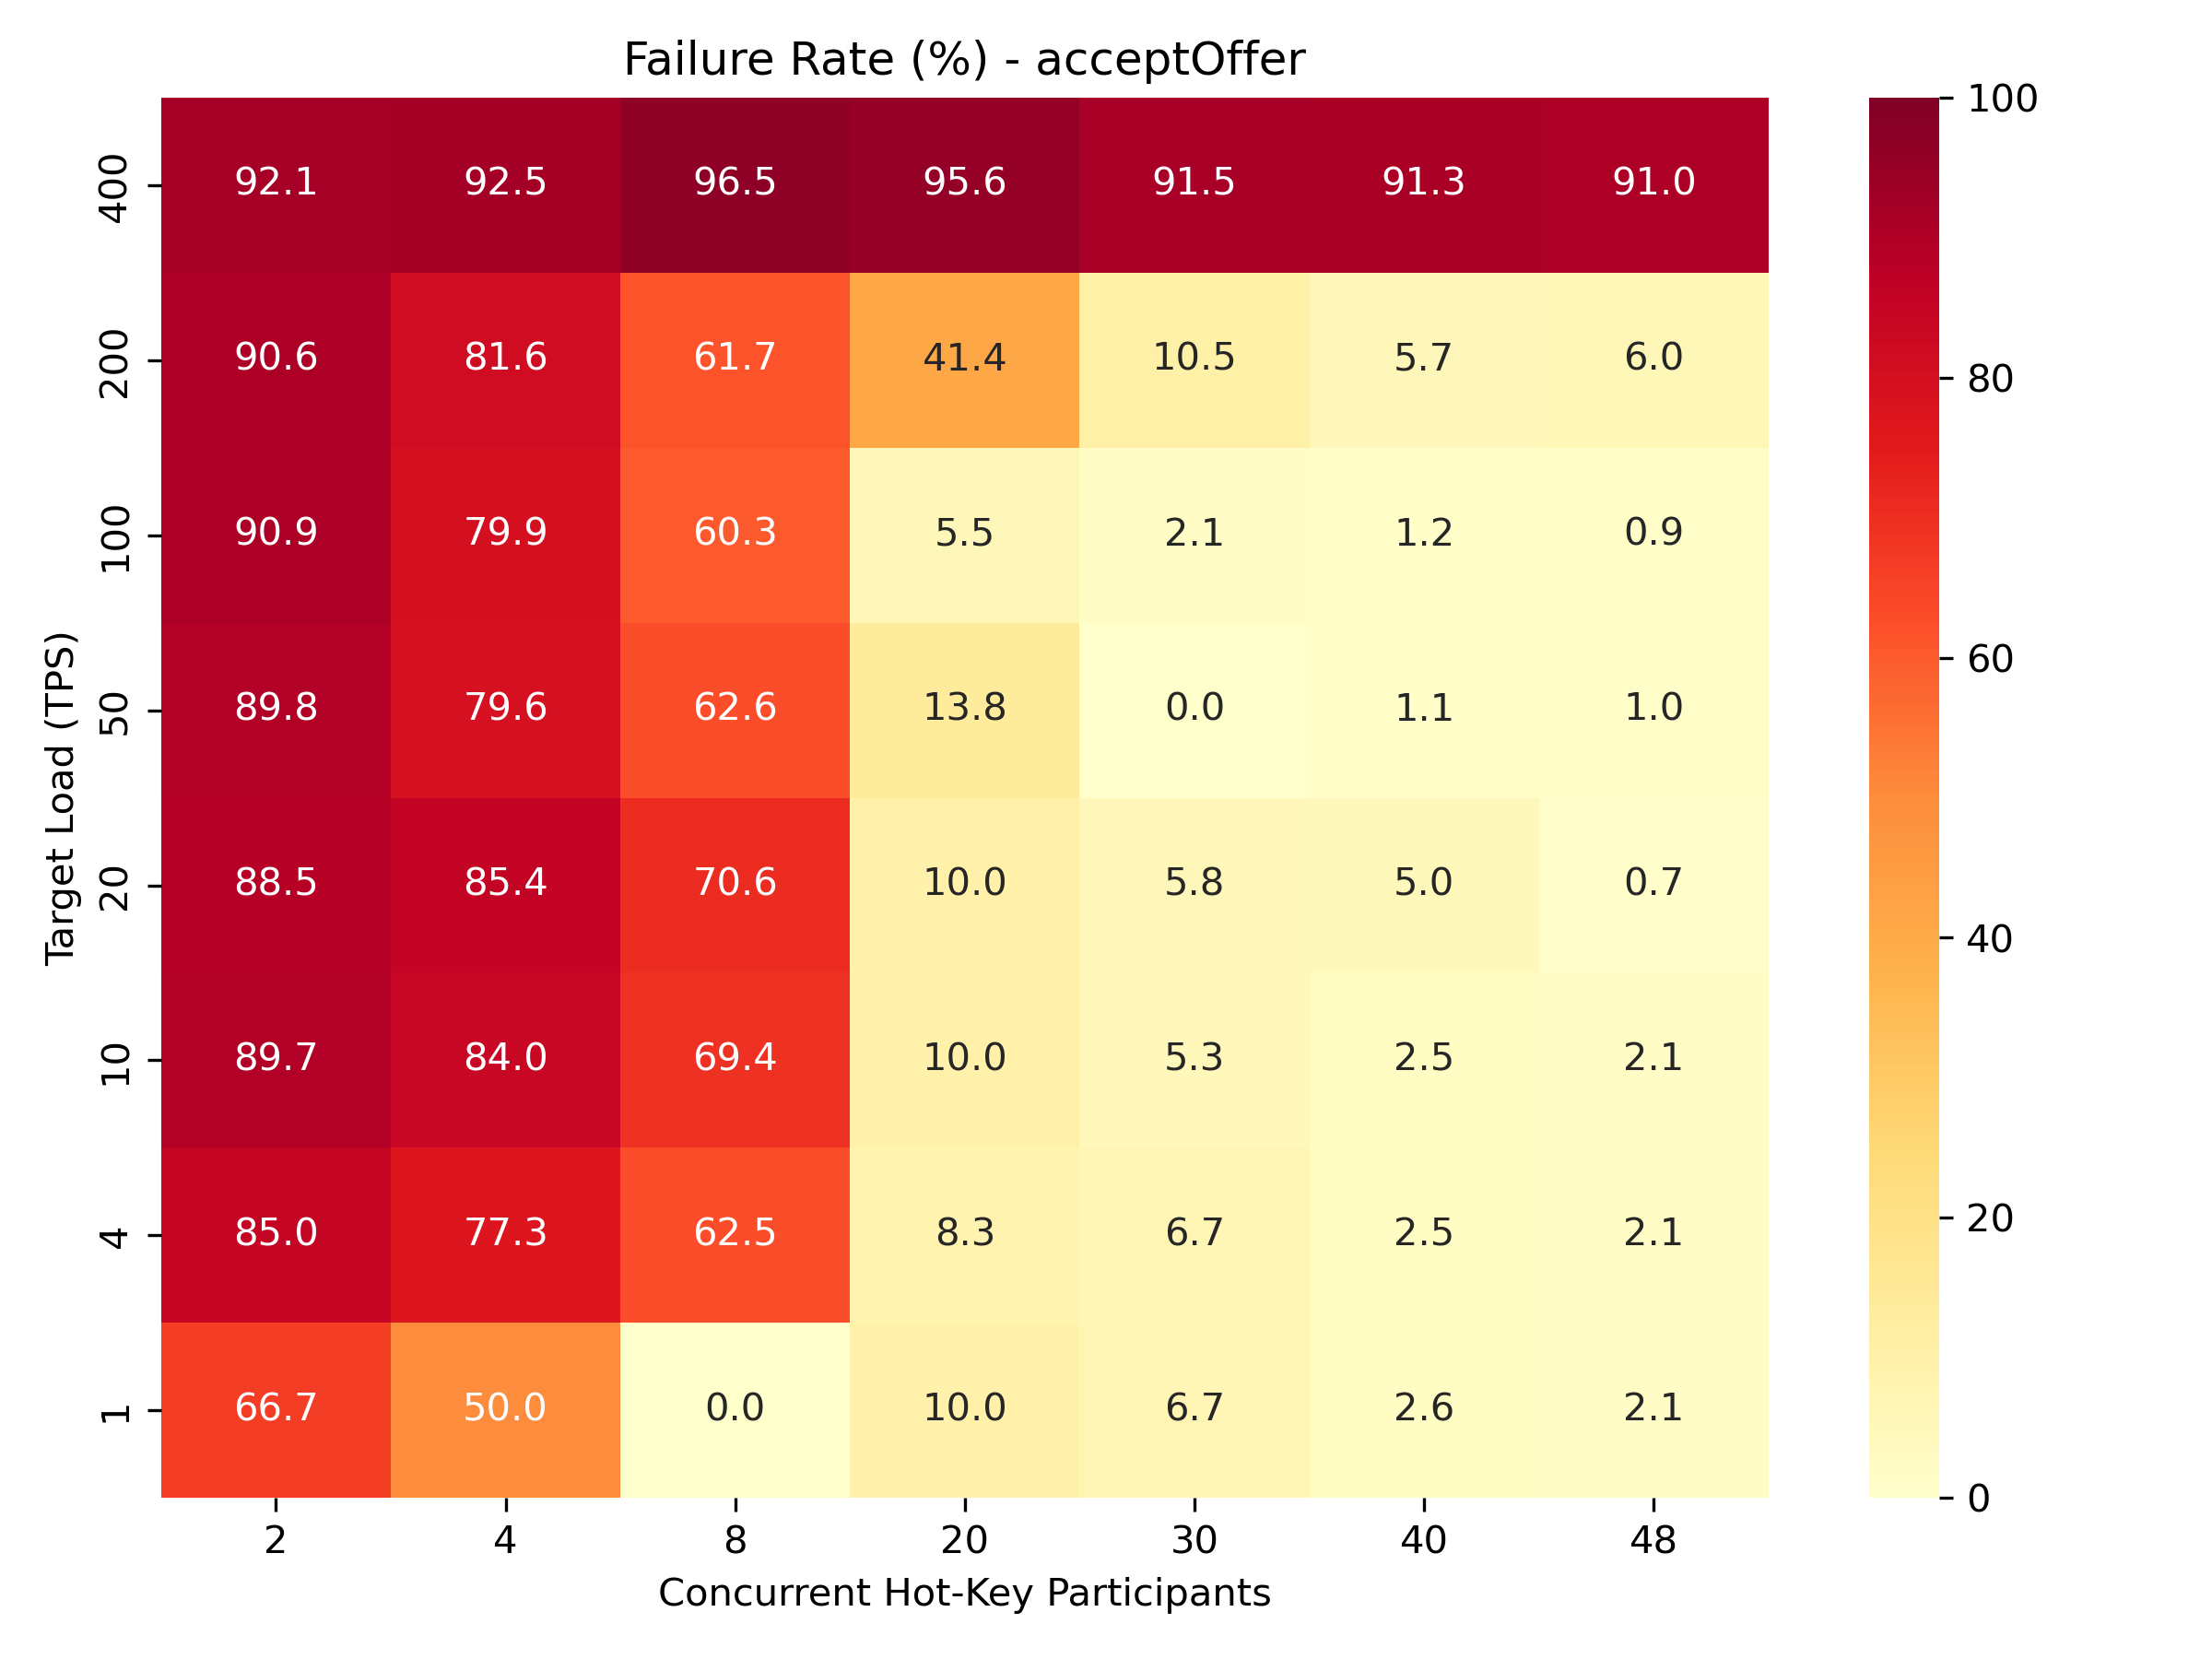
\includegraphics[width=\textwidth]{Figure_8c.png}
        \subcaption{acceptOffer}
    \end{minipage}
    \hfill
    \begin{minipage}[b]{0.48\textwidth}
        \centering
        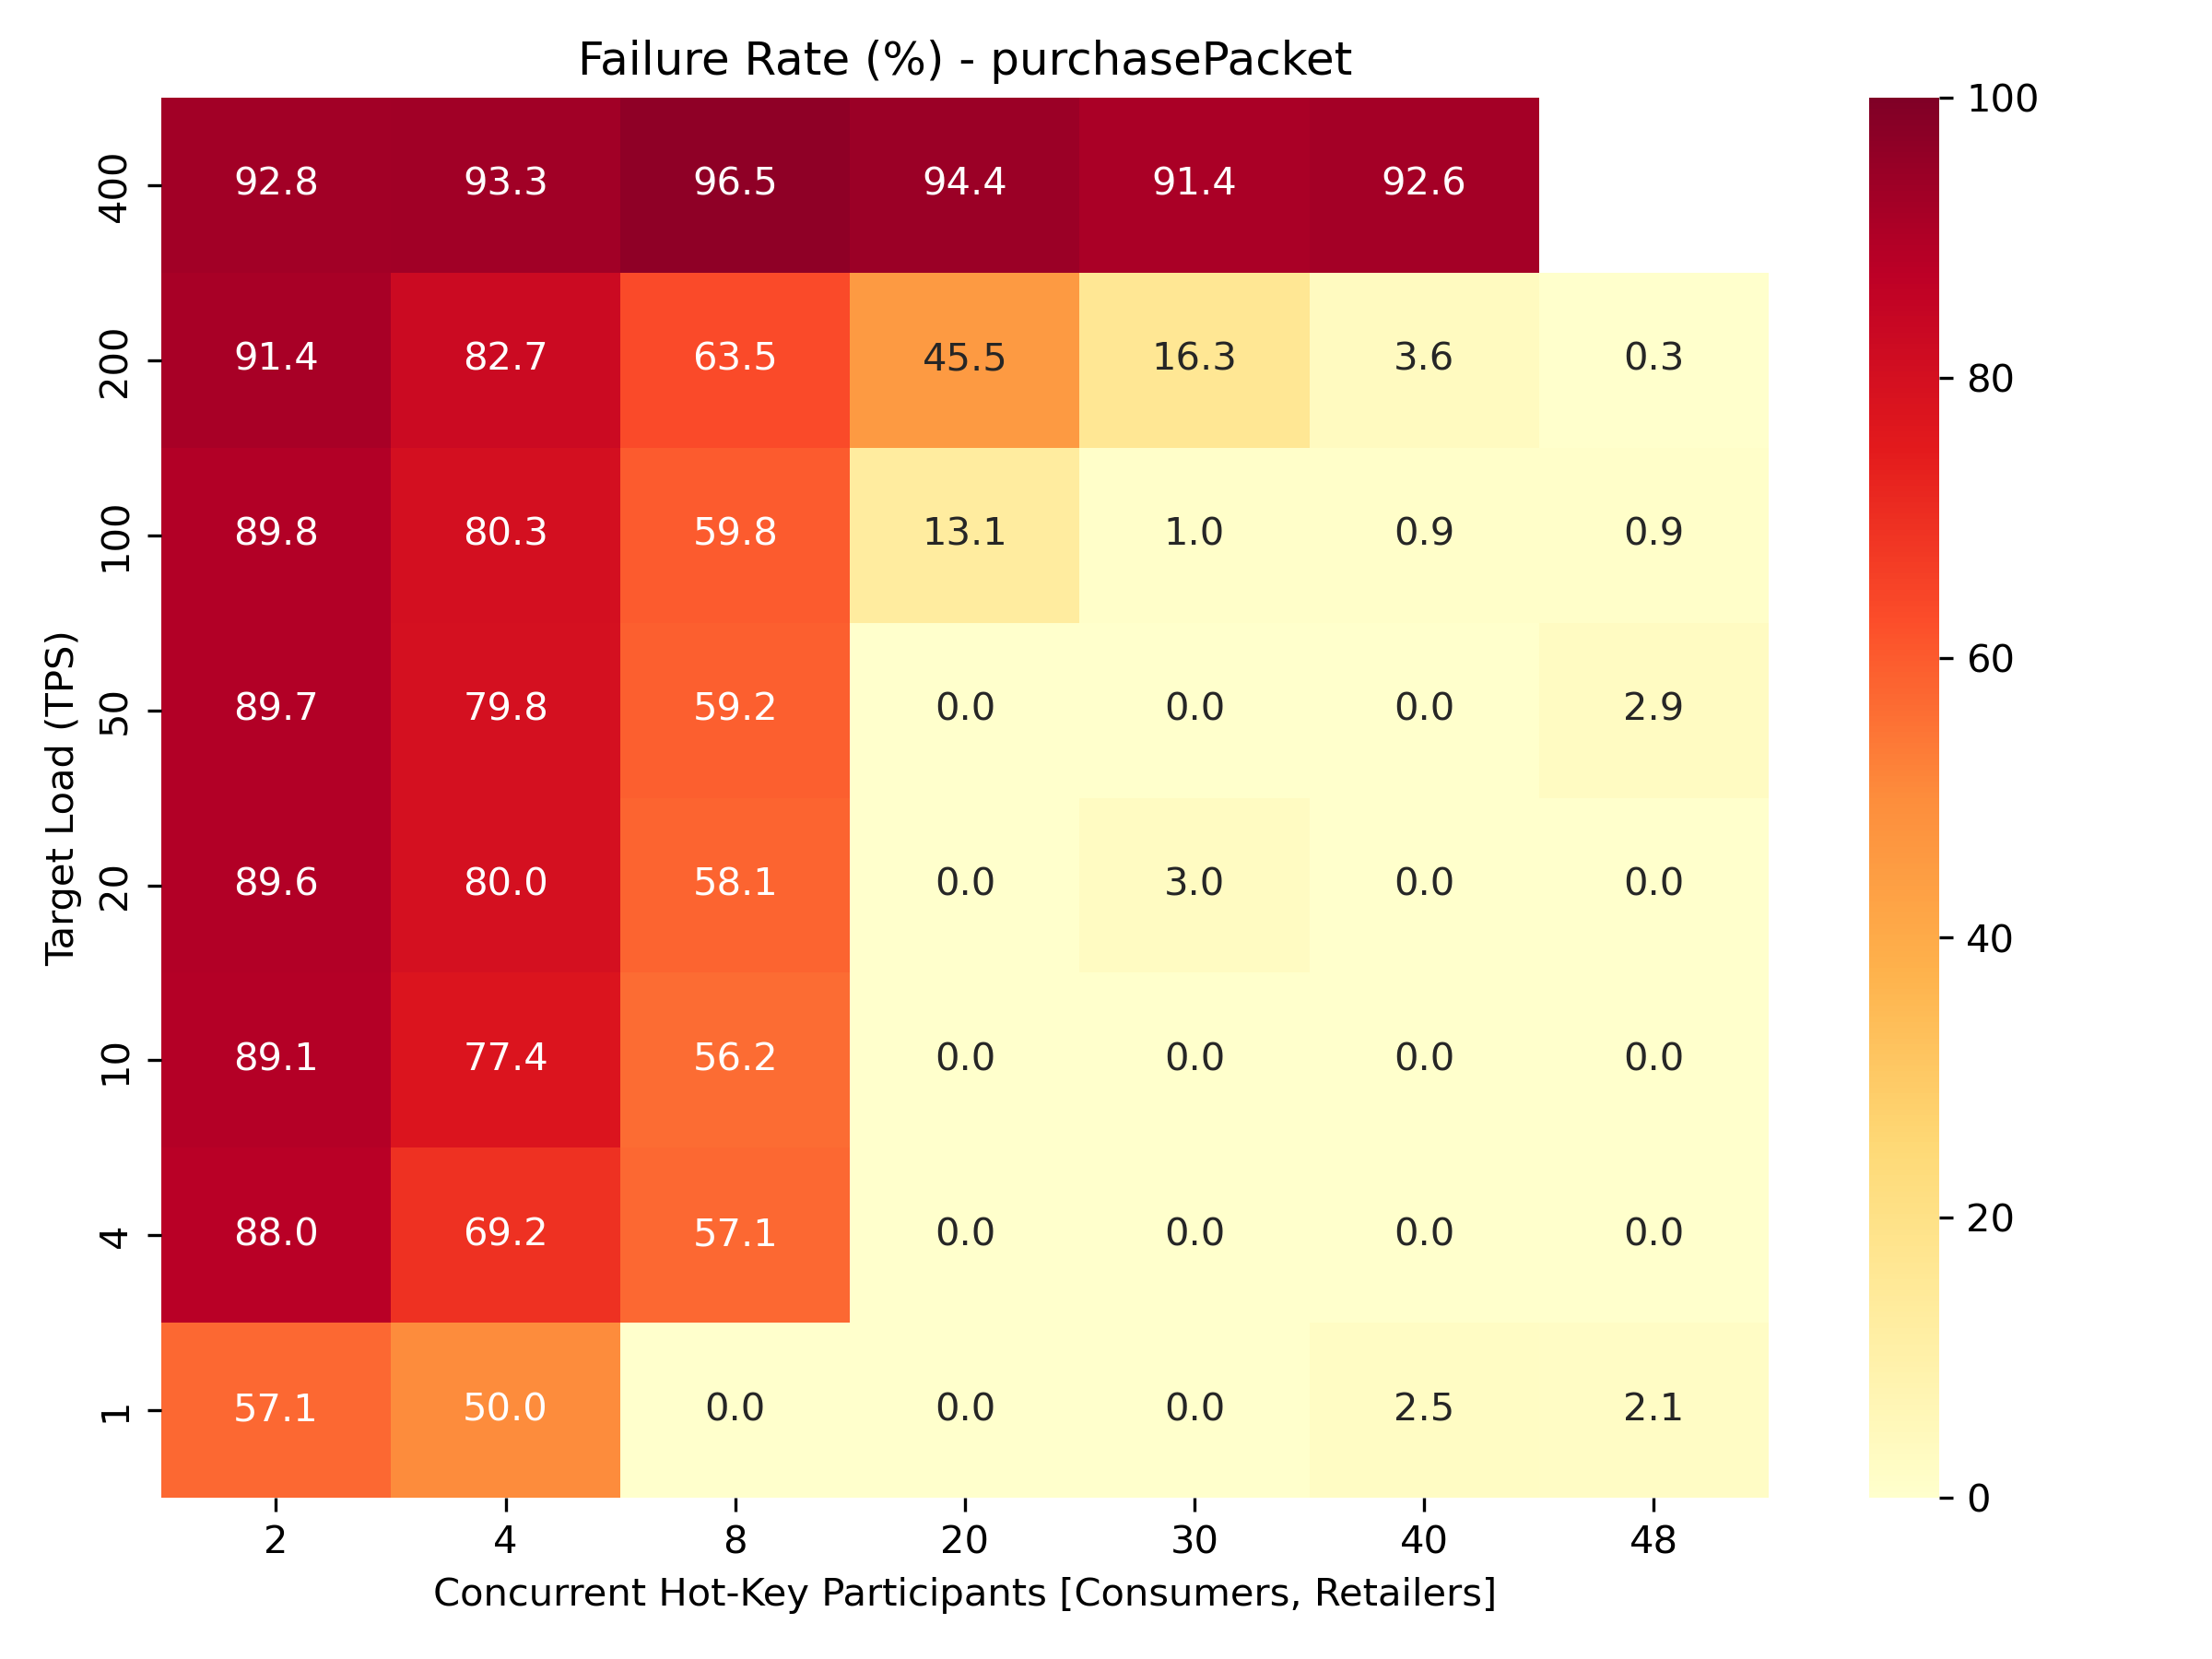
\includegraphics[width=\textwidth]{Figure_8d.png}
        \subcaption{purchasePacket}
    \end{minipage}
    \caption{Failure Rate Danger Zone matrices for the four core functions, mapping the non-linear boundaries of transaction timeouts across Target Load (TPS) and Concurrent Hot-Key Participants.}
    \label{fig:hotkey_failures}
\end{figure}

Figure \ref{fig:combined_50tps_failures} provides a cross-functional analysis of this compounding effect at a fixed load of 50 TPS. At this moderate send rate, the combination of restricted participant count and increasing network latency produced a sharp rise in failure rates across all evaluated functions. The two variables were found to be mutually reinforcing: a lower participant density intensified competition over shared ledger states, while greater latency extended the period of vulnerability to concurrent write conflicts. The combined effect consistently exceeded the impact of either variable in isolation.

\begin{figure}[H]
    \centering
    
\includegraphics[width=\textwidth]{Figure_9.png}
\caption{Transaction Failure Rate vs Network Latency and Hot-Key Contention uniformly evaluated across all core functions at exactly 50 TPS.}
    \label{fig:combined_50tps_failures}
\end{figure}







\subsection{Predictive Benchmarking}

While the empirical benchmarking characterised the performance boundaries of the supply chain chaincode, it did not fully account for the compound interactions between contributing variables. Transaction failures are governed by the joint influence of transaction load, participant density, per-transaction write complexity, and network latency. To model these interactions and identify their relative contributions, a supervised machine learning framework was applied to the Caliper benchmark dataset. The training corpus spanned participant counts from 1 to 24 and send rates from 1 to 500 TPS across all primary chaincode functions.

\begin{figure}[H]
    \centering
    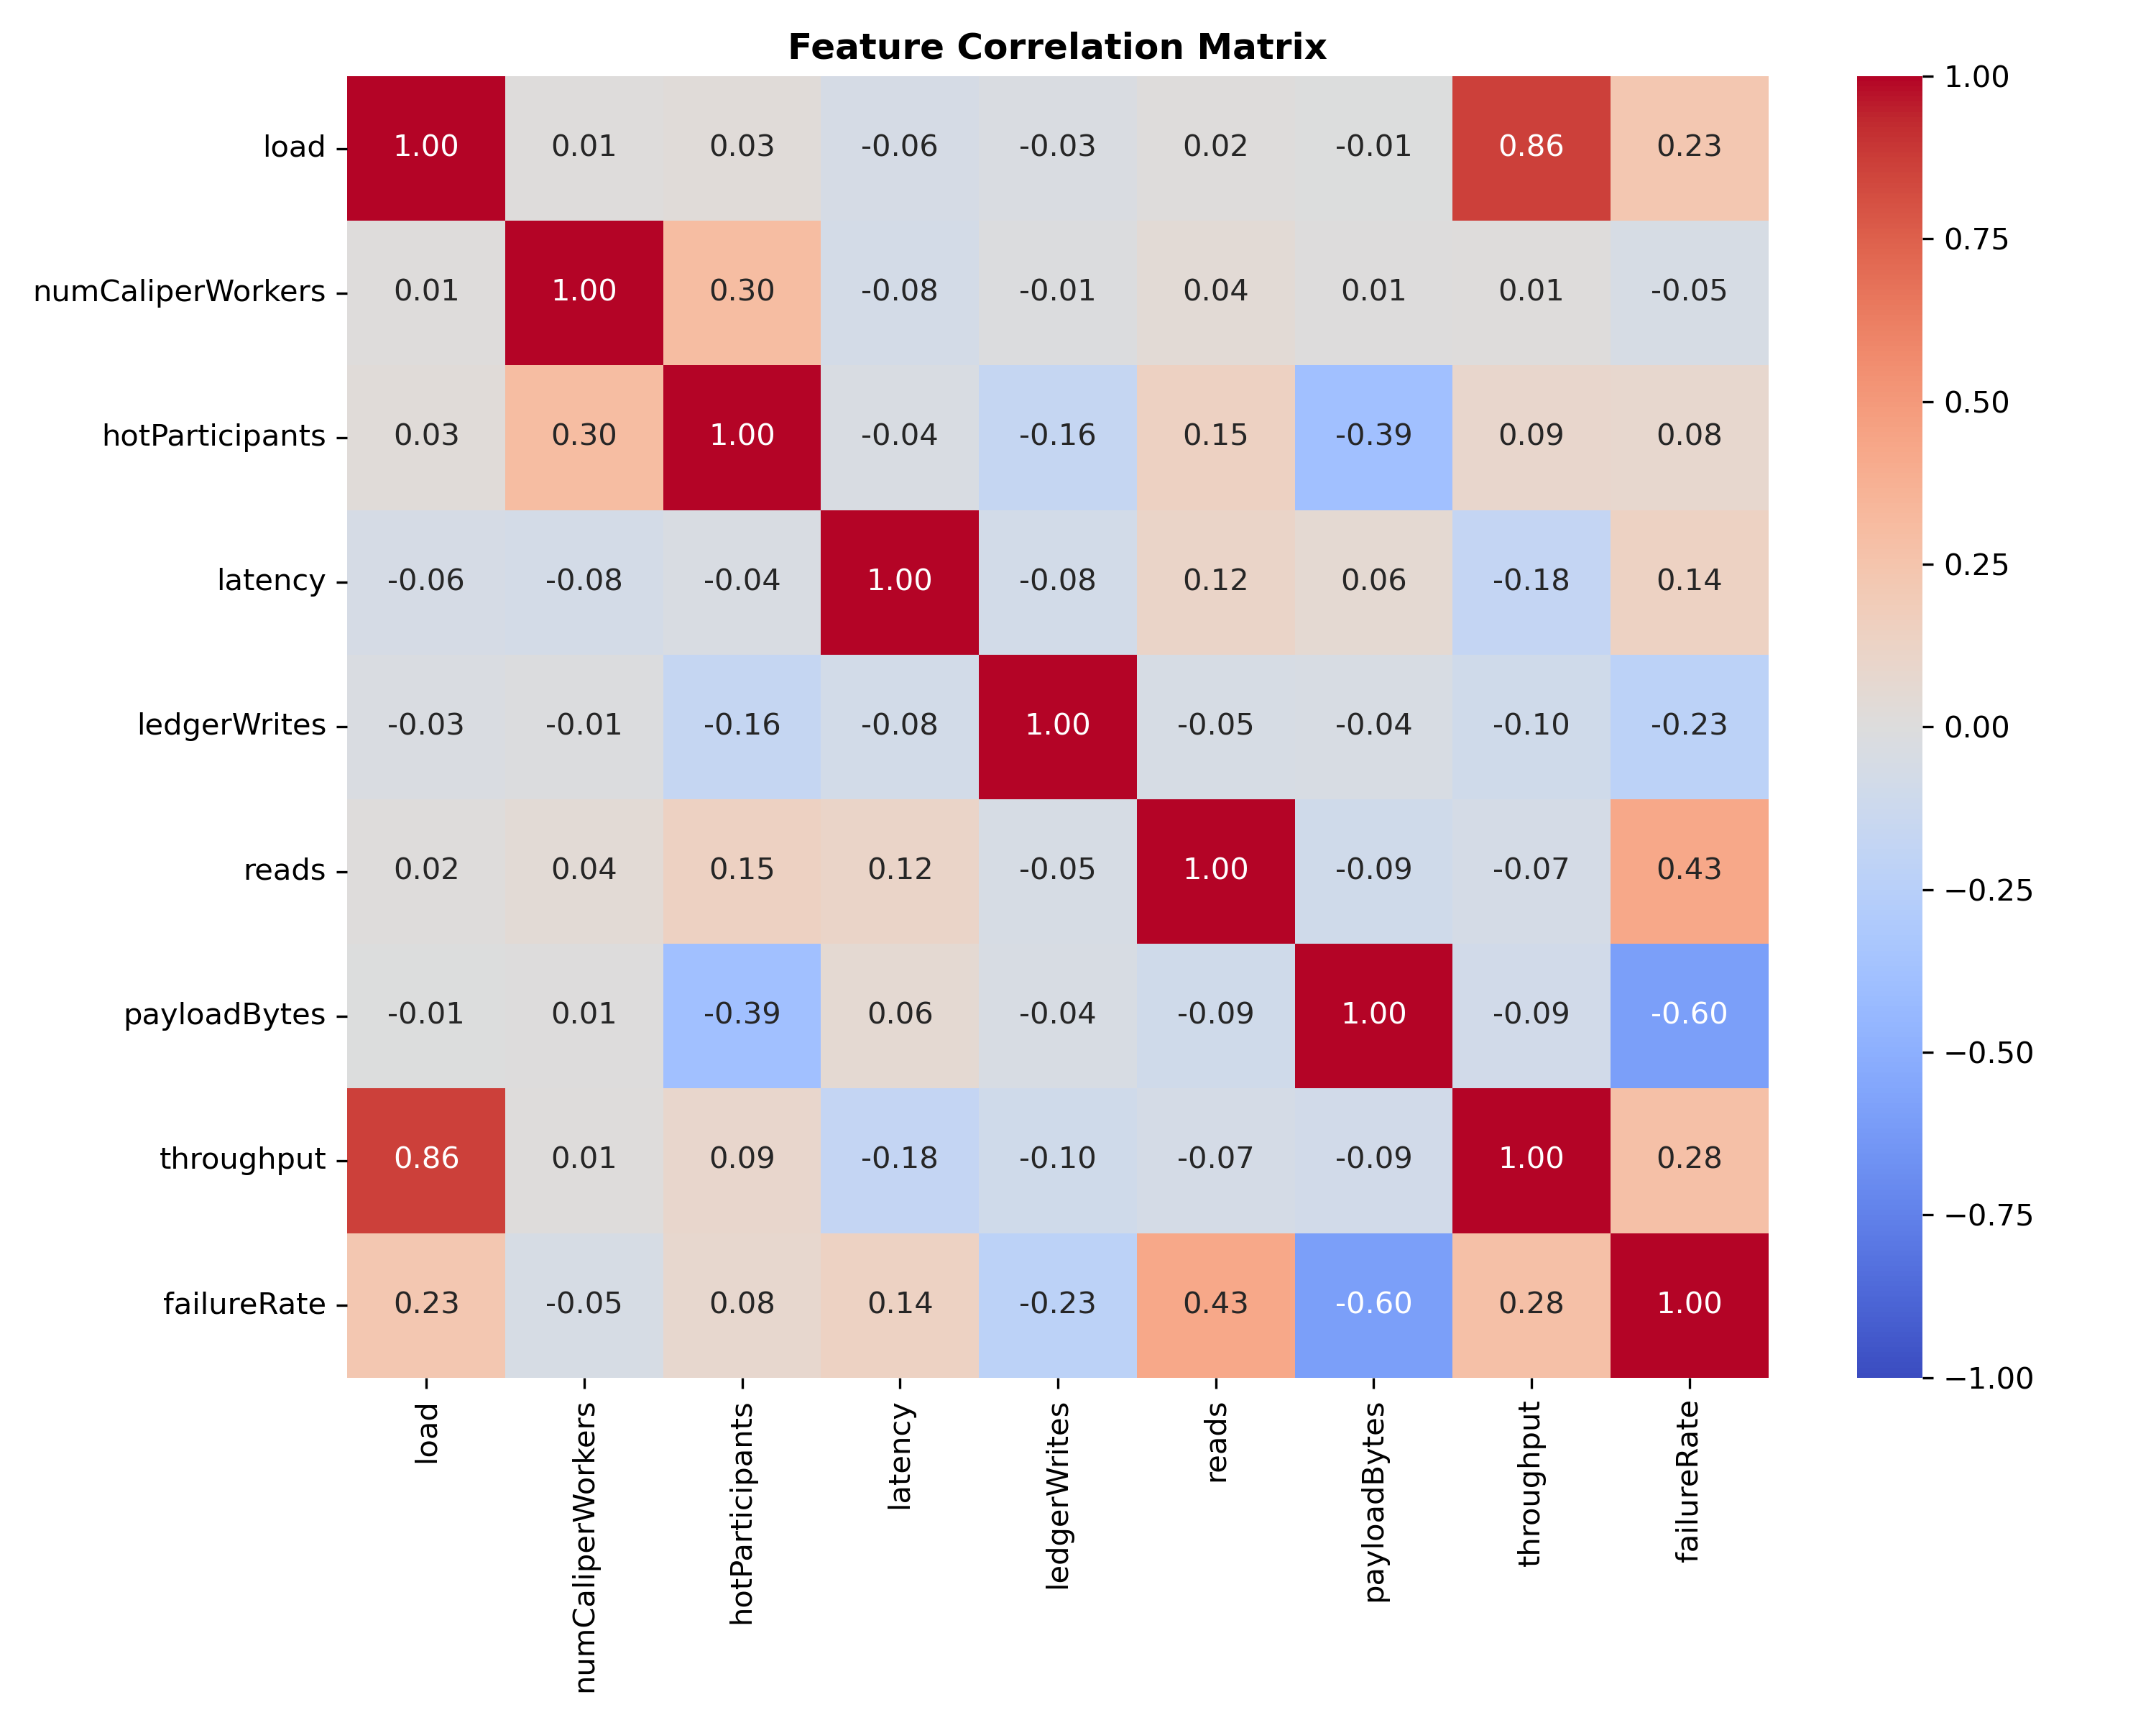
\includegraphics[width=0.8\textwidth]{Figure_10.png}
\caption{Feature Correlation Matrix showing the relationships between network variables, throughput, and failure rate.}
    \label{fig:correlation_heatmap}
\end{figure}


\subsubsection{Model Selection}
Consistent with the theoretical limitations outlined in the methodology, Linear Regression struggled to accurately model the non-linear, threshold-driven nature of MVCC transaction failures. The tree-based ensembles performed significantly better. The Random Forest regressor was selected as the primary analytical model for the remainder of this study due to its strong generalisation performance across both prediction targets and its capacity to distribute feature importance across multiple variables without disproportionate reliance on any single predictor.

\subsubsection{Throughput Prediction}
Table \ref{tab:throughput_performance} presents the comparative predictive performance of each model for transaction throughput.

\begin{table}[ht]
\centering
\caption{Comparative Predictive Performance (Target: Transaction Throughput)}
\label{tab:throughput_performance}
\resizebox{0.8\columnwidth}{!}{%
\begin{tabular}{|l|c|c|c|}
\hline
\textbf{Machine Learning Model} & \textbf{$R^2$ Score} & \textbf{MAE} & \textbf{RMSE} \\
\hline
Linear Regression & 0.8148 & 23.355 & 39.159 \\
\textbf{Random Forest Regressor} & \textbf{0.9236} & \textbf{11.933} & \textbf{25.145} \\
\hline
\end{tabular}%
}
\end{table}

The Random Forest model demonstrated strong generalisation for throughput prediction across the full experimental range. As shown in Figure \ref{fig:throughput-feature-importance}, transaction send rate (\textbf{Load}) emerged as the dominant predictor, contributing 81.1\% of the total feature importance. Secondary structural variables---\textbf{Ledger Writes} (5.7\%), \textbf{Network Latency} (5.2\%), and \textbf{Payload Bytes} (3.2\%)---each contributed meaningfully to the model's predictive capacity. These findings confirm that, while raw send rate is the primary throughput determinant, chaincode write complexity and network conditions impose measurable structural limits on attainable throughput.

\begin{figure}[H]
\centering
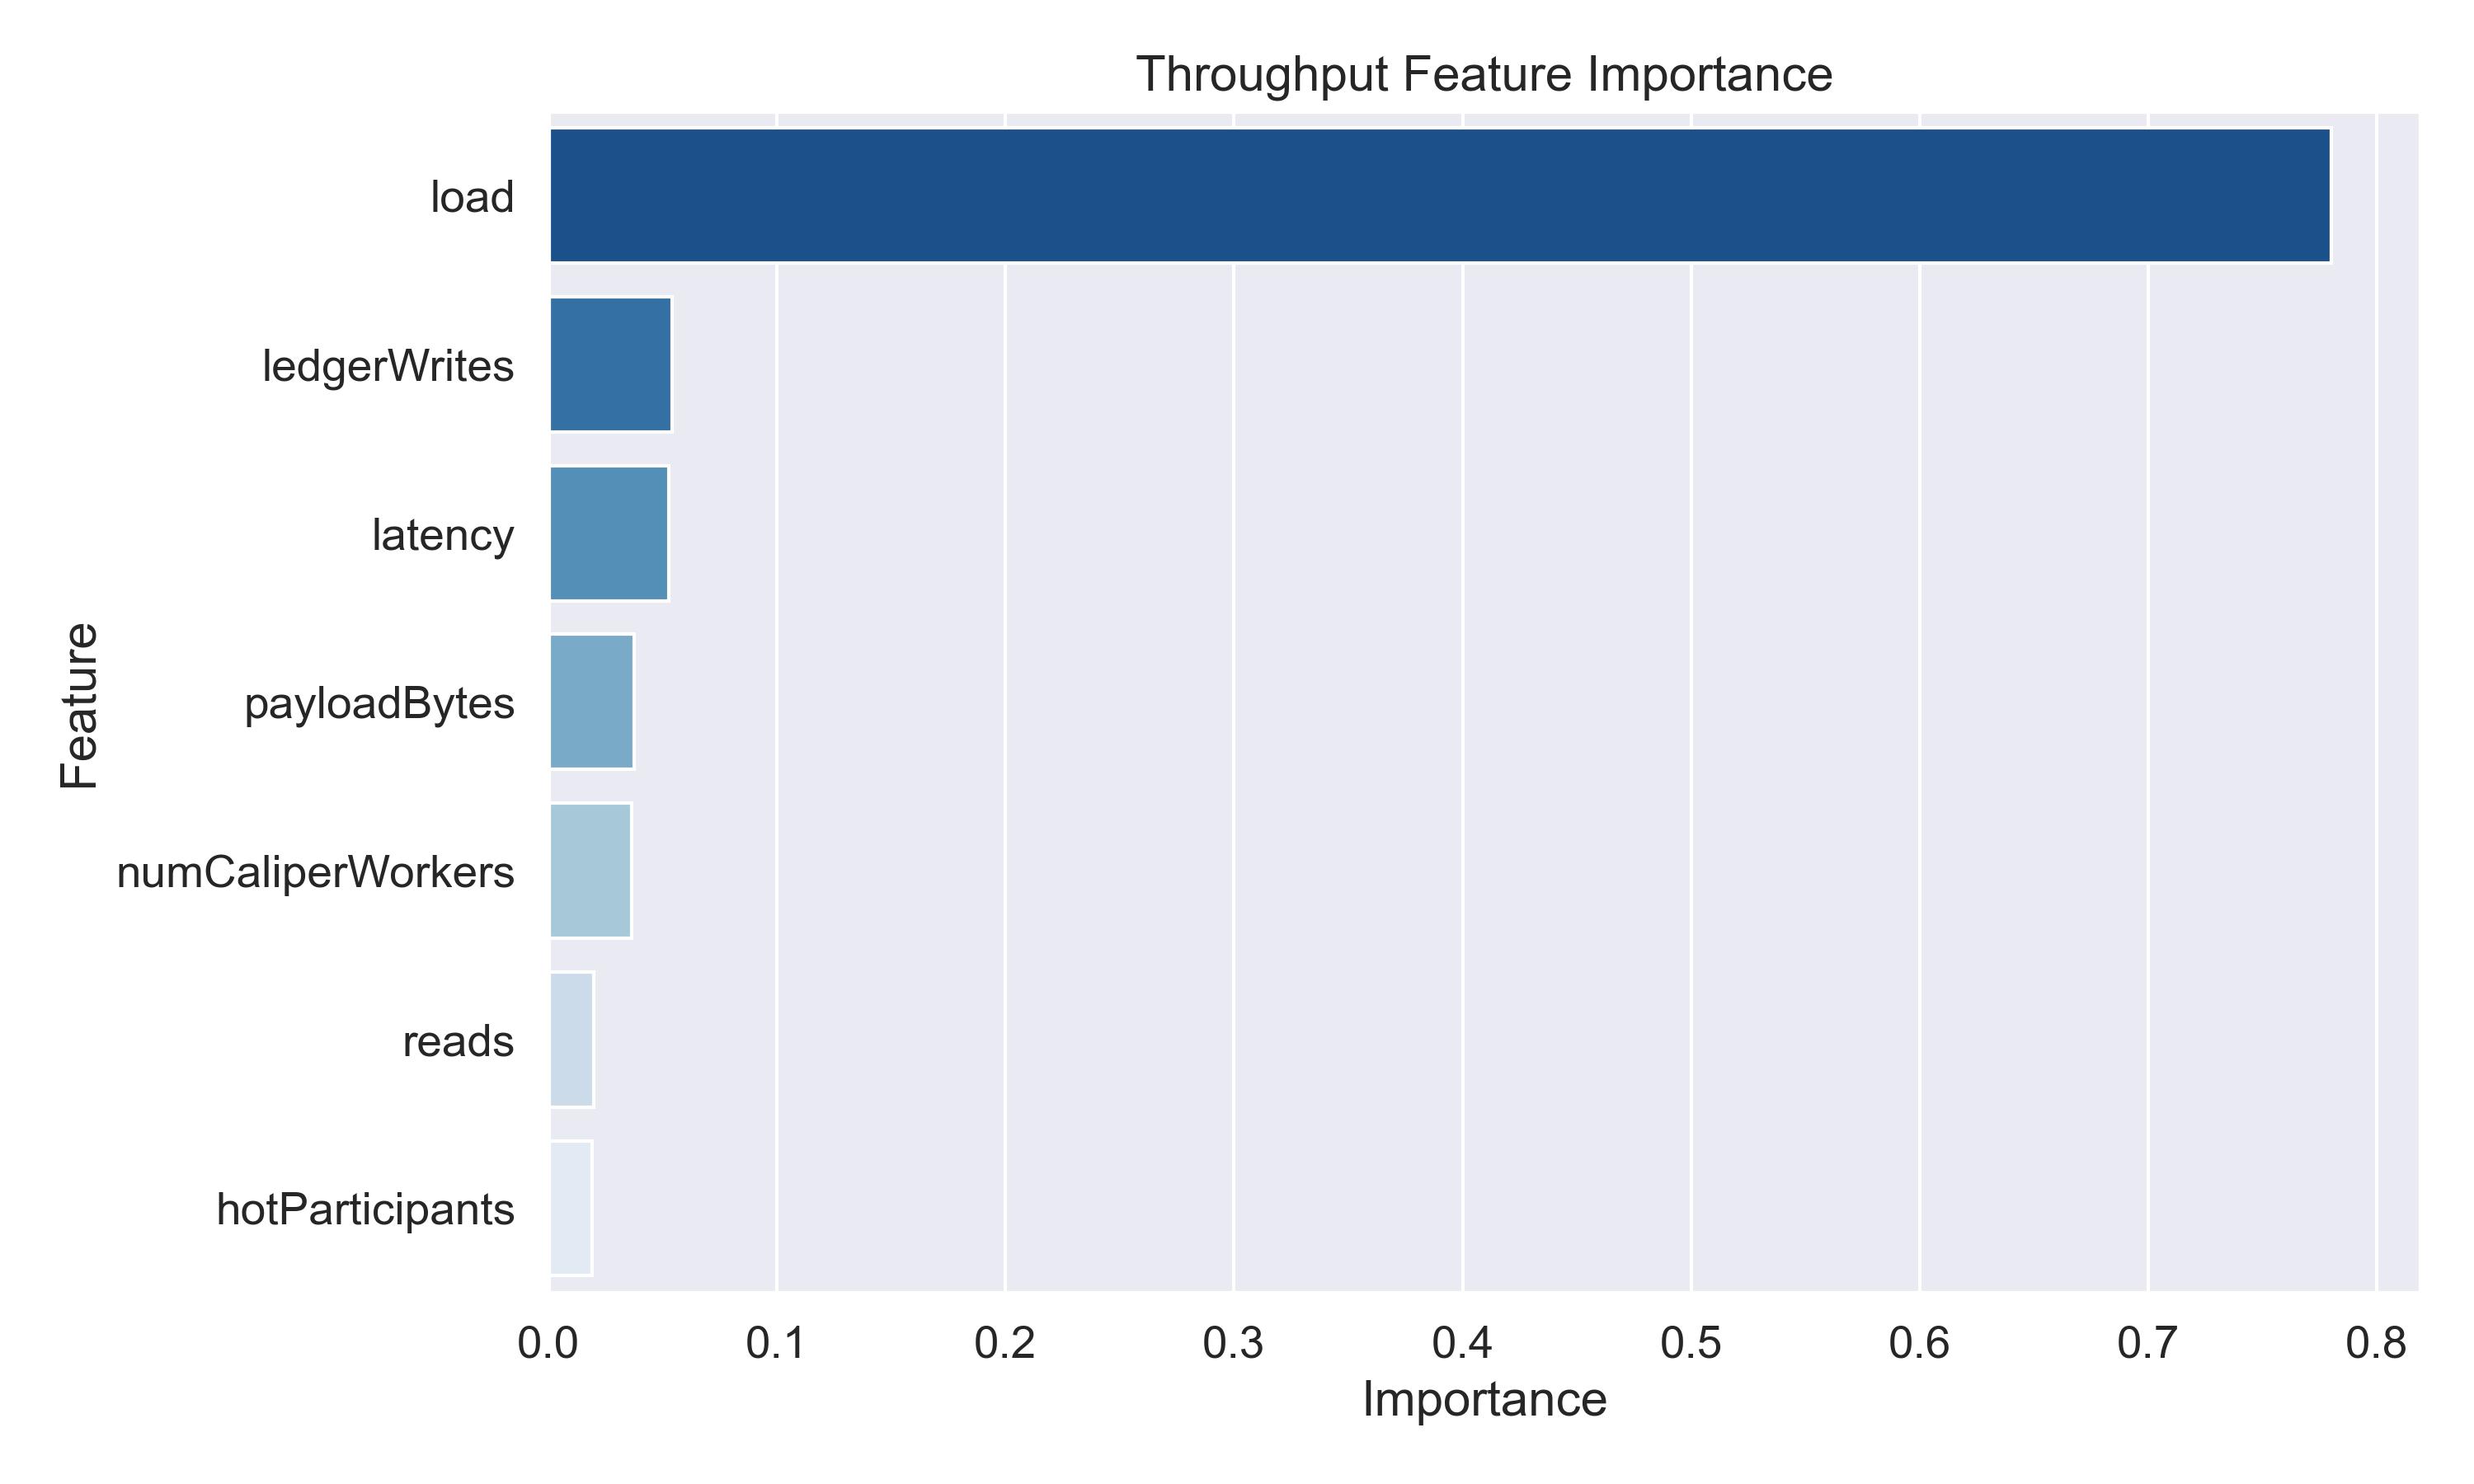
\includegraphics[width=0.8\textwidth]{Figure_11.png}
\caption{Random Forest Feature Importance ranking the dominant variables that constrain successful transaction throughput.}
\label{fig:throughput-feature-importance}
\end{figure}



\subsubsection{Failure Prediction and Feature Importance}
Table \ref{tab:failure_performance} presents the comparative predictive performance of each model for transaction failure rate.

\begin{table}[ht]
\centering
\caption{Comparative Predictive Performance (Target: Transaction Failure Rate)}
\label{tab:failure_performance}
\resizebox{0.8\columnwidth}{!}{%
\begin{tabular}{|l|c|c|c|}
\hline
\textbf{Machine Learning Model} & \textbf{$R^2$ Score} & \textbf{MAE} & \textbf{RMSE} \\
\hline
Linear Regression & 0.6680 & 0.169 & 0.224 \\
\textbf{Random Forest Regressor} & \textbf{0.9570} & \textbf{0.0368} & \textbf{0.0808} \\
\hline
\end{tabular}%
}
\end{table}

The Random Forest model yielded highly accurate predictive performance for failure rates, with results consistent with the empirical observations recorded during benchmarking. As illustrated in Figure \ref{fig:feature-importance}, the number of concurrent \textbf{Hot-Key Participants} emerged as the dominant failure predictor, accounting for 50.8\% of feature importance. This finding corroborates the empirical results: elevated participant density concentrates write operations onto a restricted set of shared ledger keys, amplifying MVCC read-write conflicts and raising the rejection rate substantially. \textbf{Payload Bytes} (20.5\%), \textbf{Transaction Load} (16.0\%) and \textbf{Network Latency} (8.7\%) ranked as the next most influential predictors. Collectively, these results indicate that transaction failure is not primarily a function of aggregate send rate, but is instead driven predominantly by the density of concurrent state contention, with payload and load acting as amplifying factors.

\begin{figure}[H]
\centering
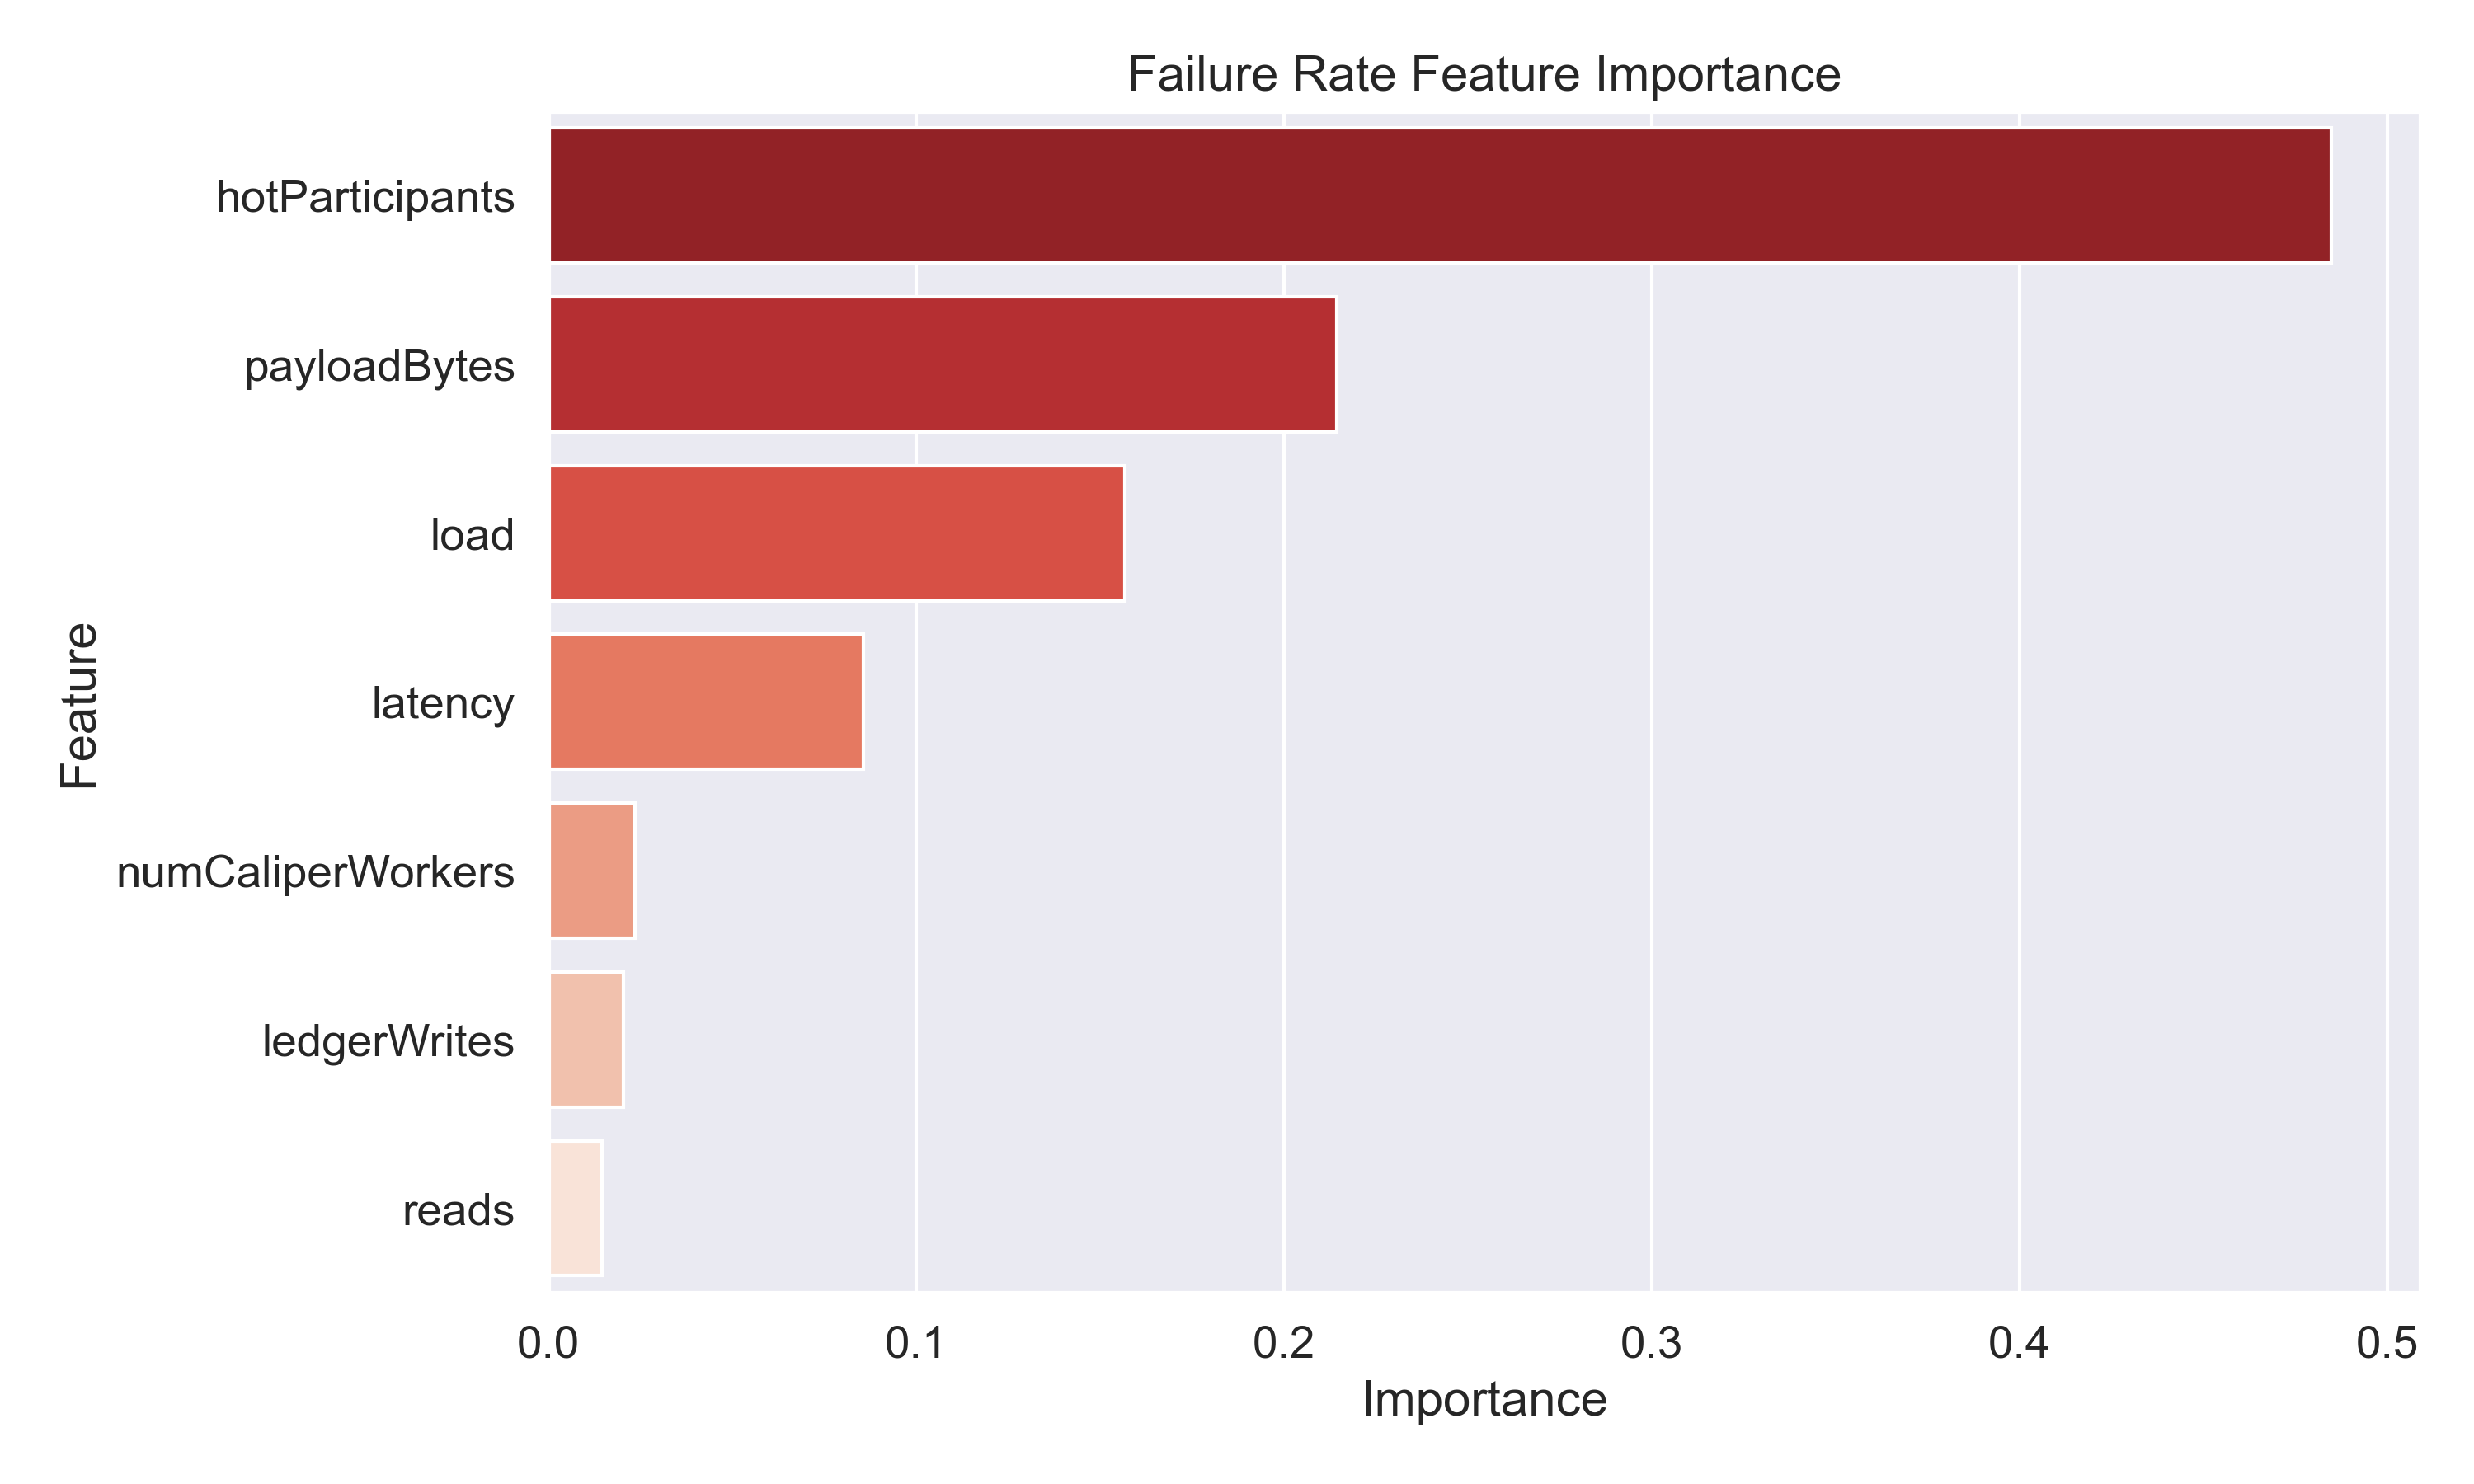
\includegraphics[width=0.8\textwidth]{Figure_12.png}
\caption{Random Forest Feature Importance ranking the distributed variables that trigger transaction failures.}
\label{fig:feature-importance}
\end{figure}



These findings indicate that mitigating transaction failure rates requires more than simply reducing the send rate. The structural design of the chaincode is a critical determinant of system resilience under concurrent access. Architectural modifications that eliminate shared write targets---such as the adoption of append-only partial composite key schemes that assign each transaction to a unique ledger slot---would directly address the primary source of MVCC contention observed throughout this study.


\section{Conclusion}
	
	This study set out to address a fundamental challenge in the practical deployment of permissioned blockchain systems: the difficulty of predicting and diagnosing non-linear Multi-Version Concurrency Control (MVCC) failures before they cause catastrophic throughput degradation in production environments. Using a Hyperledger Fabric-based agricultural supply chain system as a real-world empirical testbed, we developed and validated a machine learning framework based on Random Forest regression that accurately forecasts both MVCC failure rates and transaction throughput from interpretable structural and operational features.
	
	The supply chain system itself delivers a comprehensive permissioned blockchain platform for end-to-end traceability, smart contract-driven financial settlements, and decentralized auction-based price discovery. The system leverages a tamper-proof shared ledger to immutably record all critical lifecycle events—produce submission, quality testing outcomes, grading results, and financial transactions—ensuring transparency, accountability, and trust among all stakeholders: farmers, aggregators, retailers, banks, and consumers. The blockchain-based auction mechanism, in which each retailer bid is stored as an independent composite-key record, prevents the common MVCC hot-key bottleneck on the shared \texttt{highestOffer} field and ensures competitive, transparent price discovery. Smart contract-driven payments eliminate intermediaries, reduce settlement delays, and provide verifiable financial trails, while IPFS-based off-chain storage keeps blockchain overhead manageable.
	
	The performance analysis, conducted via Hyperledger Caliper across 11 send-rate levels and a comprehensive participant matrix, revealed severe MVCC-induced throughput degradation in functions with shared wallet keys (\textit{submitProduce}, \textit{acceptOffer}, \textit{purchasePacket}) and shared lot state (\textit{makeOffer}). Critically, the Random Forest predictive model demonstrated that \textbf{MVCC hot-key participant density} is the dominant predictor of failure rate (50.8\% feature importance), followed by payload bytes (20.5\%), transaction load (16.0\%), and network latency (8.7\%). Conversely, for throughput prediction, raw transaction load was the dominant predictor (81.1\%), with ledger writes (5.7\%) and network latency (5.2\%) acting as secondary constraints. These findings show that MVCC failures are fundamentally an architectural phenomenon driven by state-contention topology, not merely by network traffic volume.
	
	The results confirm that append-only, composite-key-based chaincode designs substantially reduce MVCC conflicts, and that the Random Forest model provides an accurate, interpretable diagnostic tool for identifying which chaincode functions and participant configurations are at highest risk. Looking ahead, future work will extend this predictive framework to distributed multi-host deployments with wide-area network conditions, explore dynamic chaincode optimization strategies guided by model predictions, and integrate real-time IoT sensor data streams for objective quality grading. The supply chain finance layer can be extended with weather-indexed smart contract insurance and credit access mechanisms leveraging verified on-chain transaction histories, further strengthening the financial resilience and scalability of agri-food blockchain deployments.
	
	\section*{Data availability}
	Data will be made available on request.
	
	\section*{Acknowledgements}
	This work was supported by \textbf{National Institute of Technology Calicut (NIT Calicut)}.
	
	
	\appendix
	

	
	
	\bibliographystyle{ACM-Reference-Format}
\bibliography{references}
	% <-- REQUIRED line
	
\end{document}

